\chapter{Authenticating Relational Queries with Fine-Grained Access Control}\label{chap:access-control}

In this chapter, we investigate the problem of authenticating relational queries with fine-grained access control. \Cref{sec:access-control:problem} introduces the formal problem definition, followed by cryptographic primitives in \cref{sec:access-control:prelim}. \Cref{sec:access-control:equality-query} presents our solution for equality queries, which is then generalized to range queries and join queries in \cref{sec:access-control:range-query} with the design of AP$^2$G-tree. A security analysis is presented in \cref{sec:access-control:security-analysis}, and \cref{sec:access-control:opt} and \cref{sec:access-control:relaxing-zero-knowledge} present optimization techniques for the zero-knowledge model and a relaxed model, respectively. How to handle duplicate records and data updates are discussed in \cref{sec:access-control:dup} and \cref{sec:access-control:update} respectively. \Cref{sec:access-control:evluation} presents the experimental results, followed by a summary in \cref{sec:access-control:summary}.

\section{Problem Formulation}\label{sec:access-control:problem}

\begin{figure}[t]
  \centering
  \resizebox{\linewidth}{!}{\begin{tikzpicture}[remember picture]
    \node (sp) {
        \begin{threeparttable}
            \begin{tabular}{|C|C|C|}
                \hline
                \multicolumn{3}{|c|}{\textbf{Database}} \\ \hline
                q\ attr. & content^{*} & \multicolumn{1}{c|}{access policy} \\ \hline
                o_1      & v_1              & Role_A \land Role_C           \\
                o_2      & v_2              & Role_A \land Role_B           \\
                o_3      & v_3              & Role_B \lor  Role_C           \\
                o_4      & v_4              & Role_C                        \\
                o_5      & v_5              & Role_A                        \\ \hline
            \end{tabular}
            \begin{tablenotes} \footnotesize
                \item[] \hspace{-0.2in} *Content is encrypted by CP-ABE
            \end{tablenotes}
        \end{threeparttable}
    };
    \node[below=0cm of sp] (sp-label) {\textbf{Service Provider (SP)}};

    \draw [red,rounded corners,thick]
    let \p1 = (sp.west),
    \p2 = ($(sp.south)!.26!(sp.north)$),
    \p3 = ($(sp.west)!.55!(sp.east)$),
    \p4 = ($(sp.south)!.59!(sp.north)$) in
    (\x1, \y2) rectangle (\x3, \y4)
    node[xshift=-0.32cm, yshift=-0.3cm] {$Q$};

    \node[matrix, left=-0.25cm of sp] {
        \node[scale=0.5] at (0,0) (do)
        {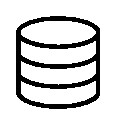
\includegraphics{figs/icons/database.eps}};
        \draw[-latex] (0,0) -- (1.8,0)
        node [above,midway,font=\footnotesize]
        {$\{(o_i, v_i, \Upsilon_i)\}$}
        node [below,midway,font=\footnotesize]
        {$ADS$};
        \\
    };
    \node[xshift=0.5cm] at (sp-label -| do) {\textbf{Data Owner (DO)}};

    \node[matrix, right=-0.25cm of sp] (users) {
        \node[scale=0.9] at (0,0) (user1) {
\includegraphics{figs/icons/user.eps}};
        \node[below=0.1cm of user1,font=\footnotesize]{$Role_A, Role_B$};
        \node[right=0cm of user1]{$u_1$};

        \node[scale=0.9] at (0,-2) (user2) {
\includegraphics{figs/icons/user.eps}};
        \node[below=0.1cm of user2,font=\footnotesize]{$Role_C$};
        \node[right=0cm of user2]{$u_2$};

        \draw[-latex,transform canvas={yshift=0.5ex}] (0, 0) -- (-2.8, 0)
        node [above,midway,font=\small] {\textcolor{red}{$Q$}};
        \draw[-latex,transform canvas={yshift=-0.5ex}] (-2.8, 0) -- (0, 0)
        node [below,midway,font=\footnotesize,align=center] {$\{\langle o_2, v_2\rangle , \langle o_3, v_3\rangle\}$ \\ $VO$};

        \draw[-latex,transform canvas={yshift=0.5ex}] (0, -2) -- (-2.8, -2)
        node [above,midway,font=\footnotesize] {\textcolor{red}{$Q$}};
        \draw[-latex,transform canvas={yshift=-0.5ex}] (-2.8, -2) -- (0, -2)
        node [below,midway,font=\footnotesize,align=center] {$\{\langle o_3, v_3\rangle , \langle o_4, v_4\rangle\}$ \\ $VO$};
        \\
    };
    \node at (sp-label -| user1) (user-label) {\textbf{Clients}};
\end{tikzpicture}
}
  \caption{Query Authentication with Access Control}\label{fig:access-control:model}
\end{figure}

As shown in \cref{fig:access-control:model}, there are three parties in the system:
\begin{inlineenum}
\item DO\@;
\item SP\@; and
\item clients.
\end{inlineenum}
The relational database $\mathcal{D}$, owned by the DO, is enforced with access control. Each record in $\mathcal{D}$ is a tuple $\langle o_i, v_i, \Upsilon_i\rangle$, where $o_i$ is the query attribute, $v_i$ is the content attribute, and $\Upsilon_i$ is the access policy. We assume that $o_i$ is discrete and distinct among all records.\footnote{The proposed approach is also applicable to continuous data which can be converted into discrete data by discretization techniques~\cite{Kotsiantis2006}. How to handle duplicate records will be discussed in \cref{sec:access-control:dup}.} We further assume that $v_i$ is encrypted by CP-ABE~\cite{10.1109/sp.2007.11} (details in \cref{sec:access-control:prelim}) for access control.\footnote{For simplicity, we assume that the query attribute is in plaintext. In cases where the query attribute is also encrypted,
privacy-preserving query techniques~\cite{10.1145/2699026.2699101} can be applied to retrieve query results, which is an orthogonal issue to query authentication.}
All the records are signed by the DO using an ADS and are outsourced to the SP, who answers queries from the clients on behalf of the DO\@.

\textbf{System Setup.}
During the system setup, the DO generates a public key ${pk}_{client}$ (CP-ABE encryption key) and a secret key ${sk}_\text{DO}$ (ABS signing key), which can be used to encrypt the data and generate the ADS, respectively. The DO also distributes a secret key ${sk}_{client}$ (CP-ABE decryption key) and a public key ${pk}_\text{DO}$ (ABS verification key) to the clients, who can use them to decrypt and verify the query results, respectively.

\textbf{Access Policy.}
Access policies control the results of a query with respect to the roles of the client.\footnote{We use ``roles'' and ``attributes'' interchangeably in the context of ABE and ABS.}
For example, given the same range query $Q$ in \cref{fig:access-control:model}, the result set to client $u_1$ with $Role_A$ and $Role_B$ is $\{\langle o_2, v_2\rangle$, $\langle o_3, v_3\rangle\}$ and that to client $u_2$ with $Role_C$ is $\{\langle o_3, v_3\rangle$, $\langle o_4, v_4\rangle\}$. In general, an access policy can be viewed as a boolean function in the form of $\Upsilon : {\{0, 1\}}^n \to \{0, 1\}$. It accepts multiple boolean inputs, each corresponding to a role, and outputs 1 or 0. For example, if $\Upsilon$ is defined as $({Role}_A \land {Role}_C) \lor {Role}_B$, then $\Upsilon({Role}_A) = 0$ and $\Upsilon({Role}_B, {Role}_C) = 1$. Here, for clarity, we omit those inputs with zero values (e.g., a singleton $Role_A$ implies that $Role_B$ and $Role_C$ are missing). While, technically, an access policy can take any boolean function, in the literature, most works focus on a specific type, namely, monotone boolean functions~\cite{10.1145/1180405.1180418,10.1109/sp.2007.11,10.1007/978-3-642-19074-2_24,10.1145/1755688.1755697}. Formally, the monotonic property means that, for all $a_i$ and $b_i$ in $\{0, 1\}$, if $a_1 \le b_1$, $\dots$, $a_n \le b_n$, then $\Upsilon(a_1, \dots, a_n) \le \Upsilon(b_1, \dots, b_n)$ holds. This property suggests that a client with more roles has a higher clearance level and so can access more data. % chktex 8
For simplicity, we assume that all access control policies are monotone boolean functions that are normalized in a \emph{disjunctive normal form} (DNF).

\textbf{Threat Model.}
Two security threats are considered in our problem:
\begin{inlineenum}
\item the SP is not fully trusted and it might return tampered or incomplete query results; and
\item the clients are curious and may want to learn the information about the data to which access is unauthorized.
\end{inlineenum}

To address the first threat, we advocate authenticated query processing. Specifically, during query processing, the SP traverses the ADS and constructs a VO that includes the verification information of the results. The VO is returned to the client along with the results. Using the VO, the client should establish the \emph{soundness} and \emph{completeness} of a result set $RS$:
\begin{itemize}
  \item \textbf{Soundness}. No records in $RS$ are tampered with and are truly the results with respect to the roles of the client.
  \item \textbf{Completeness}. All records not in $RS$ are either non-results or are inaccessible to the client.
\end{itemize}
Take the range query $Q$ in \cref{fig:access-control:model} as an example. $RS=\{\langle o_2, v_2\rangle$, $\langle o_3, v_3\rangle\}$ is the correct result set for client $u_1$. $RS_1 = \{\langle o_2, v_2'\rangle$, $\langle o_3, v_3\rangle\}$ and $RS_2 = \{\langle o_2, v_2\rangle$, $\langle o_3, v_3\rangle$, $\langle o_4, v_4\rangle\}$ are not sound because they either contain fake ($v_2'$ in $RS_1$) or inaccessible ($o_4$ in $RS_2$) records. $RS_3 = \{\langle o_2, v_2\rangle\}$ is not complete because $o_3$ is missing.

To further address the second threat, we need to protect data access against unauthorized clients during query authentication. We define three levels of confidentiality requirements:
\begin{itemize}
  \item \textbf{Data Content Confidentiality}. The contents of inaccessible records are protected. This is a basic requirement for any query service that supports access control.
  \item \textbf{Access Policy Confidentiality}. In addition to data content confidentiality, the access policies of inaccessible records are protected. That is, the clients must not know that their denied access is due to the lack of some specific role(s). % chktex 36
  \item \textbf{Zero-Knowledge Confidentiality}.
    Any information beyond the accessible records $\mathcal{D}^+$ in the database $\mathcal{D}$ is protected. That is, the clients can gain nothing about $\mathcal{D}\backslash\mathcal{D}^+$ (e.g., not even its size or the associated access policies).
\end{itemize}
The above security notions will be formalized when we perform security analysis in \cref{sec:access-control:security-analysis-query}. We assume that there is no collusion between the SP and clients.

In what follows, we propose a zero-knowledge query authentication solution that addresses both of the security threats under fine-grained access control. We will develop new query authentication techniques for ADS generation, VO construction, and result verification that achieve the zero-knowledge confidentiality. To cater for performance-centric applications, we will also discuss how to further improve the query authentication performance by relaxing the confidentiality requirement.

\section{Preliminaries}\label{sec:access-control:prelim}

This section gives some preliminaries on cryptographic constructs and integrity assurance.

\textbf{Cryptographic Hash Function.}
A cryptographic hash function $H(\cdot)$ accepts an arbitrary-length string as its input and returns a fixed-length bit string. It is collision resistant; it is difficult to find two different messages, $m_1$ and $m_2$, such that $H(m_1) = H(m_2)$. Classic cryptographic hash functions include the SHA-1, SHA-2, and SHA-3 family.

\textbf{Bilinear Pairing.}
Bilinear pairing maps a pair of elements in two groups to a single element in a third group, which serves as a basic operation in \emph{attribute-based encryption} (ABE) and \emph{attribute-based signature} (ABS), as shown later in this chapter.

Let $\mathbb{G}$, $\mathbb{H}$, and $\mathbb{G}_T$ be three cyclic multiplicative groups with the same order $p$, where $p$ is a prime. Let $g$, $h$ be the generator of $\mathbb{G}$ and $\mathbb{H}$, respectively. We can find a bilinear mapping $e: \mathbb{G} \times \mathbb{H} \rightarrow \mathbb{G}_T$, which has the following properties:
\begin{itemize}
  \item \textsf{Bilinearity}: If $u \in \mathbb{G}$, $v \in \mathbb{H}$, and $e(u,v)\in\mathbb{G}_T$, then $e(u^a, v^b) = {e(u, v)}^{ab}$ for any $u,v$.
  \item \textsf{Non-degeneracy}: $e(g, h) \neq 1$.
\end{itemize}

\textbf{Ciphertext-Policy Attribute-Based Encryption (CP-ABE).}
CP-ABE is proposed to realize complex access control over encrypted data~\cite{10.1109/sp.2007.11}. By embedding the access policy into the ciphertext, it enables fine-grained access control represented by a boolean function of attributes.
It consists of a set of algorithms:
\begin{itemize}
  \item \textsf{CP-ABE.Setup}$(1^\lambda) \to (mk, pp)$:
    On input a security parameter $1^\lambda$, it generates a master private key $mk$ and a public key $pp$.
  \item \textsf{CP-ABE.KeyGen}$(mk, \mathcal{A}) \to {sk}_\mathcal{A}$:
    On input a master private key $mk$ and an attribute set $\mathcal{A}$, it outputs a decryption key ${sk}_\mathcal{A}$.
  \item \textsf{CP-ABE.Encrypt}$(pp, x, \Upsilon) \to c_{\Upsilon}$:
    On input a public key $pp$ and an access policy $\Upsilon$, it encrypts plaintext $x$ into ciphertext $c_\Upsilon$.
  \item \textsf{CP-ABE.Decrypt}$({sk}_\mathcal{A}, c_\Upsilon) \to x$:
    On input a decryption key ${sk}_\mathcal{A}$, ciphertext $c_\Upsilon$, it outputs plaintext $x$ if $\Upsilon(\mathcal{A}) = 1$; otherwise $\bot$ is returned.
\end{itemize}

\textbf{Attribute-Based Signature (ABS).}
Introduced in~\cite{10.1007/978-3-642-19074-2_24}, ABS is a signature scheme that enables a party to sign a message with fine-grained access control over the identifying information. Unlike a traditional signature scheme, messages can be signed with a monotone boolean function predicate that is satisfied by the attributes obtained from the authority. It consists of the following algorithms:
\begin{itemize}
  \item \textsf{ABS.Setup}$(1^\lambda) \to (msk, mvk)$:
    On input a security parameter $1^\lambda$, it generates a master signing key $msk$ and a master verification key $mvk$.
  \item \textsf{ABS.KeyGen}$(msk, \mathcal{A}) \to {sk}_\mathcal{A}$:
    On input a master signing key $msk$ and an attribute set $\mathcal{A}$, it outputs a signing key ${sk}_\mathcal{A}$.
  \item \textsf{ABS.Sign}$({sk}_\mathcal{A}, m, \Upsilon) \to \sigma_{m,\Upsilon}$:
    On input a signing key ${sk}_\mathcal{A}$, a message $m$, and a monotone boolean function predicate $\Upsilon$, where $\Upsilon(\mathcal{A}) = 1$, it outputs a signature $\sigma_{m,\Upsilon}$.
  \item \textsf{ABS.Verify}$(mvk, m, \Upsilon, \sigma_{m,\Upsilon}) \to \{0, 1\}$:
    On input a master verification key $mvk$, an unverified message $m$, an unverified monotone boolean function predicate $\Upsilon$, and a signature $\sigma_{m,\Upsilon}$, it outputs 1 if the signature is valid.
\end{itemize}

More elaborate procedures, along with extended algorithms, will be given in \cref{sec:access-control:abs}.

\section{Equality Query Authentication}\label{sec:access-control:equality-query}

A naive solution to query authentication with fine-grained access control is to use the Merkle hash tree~\cite{10.1007/0-387-34805-0_21} to construct a VO for authenticated query processing and to use CP-ABE to encrypt data records for access control. More specifically, for any query, all data records (including those inaccessible ones) that lie in the query range, along with the VO, are returned to the client. After verifying the records, the client can decrypt and access the authorized records, using the attribute secret key obtained from the DO\@. However, this solution has two problems. First, it will return a large number of inaccessible records to the client, which incurs high computation and communication overheads. Second, for the inaccessible records, thanks to CP-ABE, although they cannot be decrypted by the client, returning them still reveals some information about their existence and their access policies. This violates our zero-knowledge confidentiality requirement.

In the following, we propose new query authentication techniques that support both fine-grained access control and zero-knowledge confidentiality. We start with equality queries by developing a novel signature scheme in this section and then extend it to range queries and join queries in \cref{sec:access-control:range-query}.

In an equality query, the client specifies a query key $o_q$ as well as his/her access role set $\mathcal{A}$. Since the query attribute is distinct, there could be three possible outcomes:
\begin{itemize}
  \item There is one record matching $o_q$ and it is accessible to the query client.
  \item There is one record matching $o_q$ but it is not accessible to the query client.
  \item There is no record matching $o_q$.
\end{itemize}

Recalling our zero-knowledge confidentiality does not allow the client to distinguish between the last two outcomes. To prevent the information leakage caused by non-existent records, we introduce a global pseudo access role, ${Role}_{\emptyset}$, which is not possessed by any client. We treat each non-existent record as a \emph{pseudo} record that is associated with the access policy ${Role}_{\emptyset}$. As such, for any equality query, there is always one matching record with one of the two possible outcomes: accessible or inaccessible.

\subsection{ADS Generation and Query Processing}

\textbf{ADS Generation.} Our construction for zero-knowledge query authentication is built upon a novel signature scheme. During the system setup, the DO generates a signature for each data record. These signatures, serving as ADS, are sent to the SP, who will then use them to support verifiable queries. As mentioned earlier, the signature has two design requirements. First, given a record $i$, the signature should capture all of its three components (query attribute $o_i$, data content $v_i$, and access policy $\Upsilon_i$) so that it can be used as a proof of integrity. Second, in case the record is inaccessible to some clients, the signature can be tailored to prove the inaccessibility with the zero-knowledge confidentiality. To this end, we propose a new access-policy-preserving (APP) signature based on a variant of the ABS (to be detailed in \cref{sec:access-control:abs}).

\begin{definition}[APP Signature] Consider a record $\langle o_i$, $v_i$, $\Upsilon_i\rangle$. Let ${sk}_{\textrm{DO}}$ be the signing key of the DO, $H(\cdot)$ a cryptographic hash function, and `$|$' denote string concatenation. The access-policy-preserving (APP) signature for this record is generated as:
  \begin{align*}
    \sigma_i & = \textsf{ABS.Sign}({sk}_{\textrm{DO}}, H(o_i) | H(v_i) , \Upsilon_i)
  \end{align*}
  In the case of pseudo (non-existent) records, $v_i$ will be assigned a random value and $\Upsilon_i$ will be ${Role}_{\emptyset}$.
\end{definition}

\begin{figure}[t]
  \centering
  \resizebox{\linewidth}{!}{\begin{tikzpicture}
    \node[matrix] (users) {
        \node[scale=0.9] at (0,0) (user1) {
\includegraphics{figs/icons/user.eps}};
        \node[below=0cm of user1]{$Role_A, Role_B$};
        \node[right=0cm of user1]{$u_1$};

        \node[scale=0.9] at (0,-2) (user2) {
\includegraphics{figs/icons/user.eps}};
        \node[below=-0.1cm of user2]{$Role_C$};
        \node[right=-0.1cm of user2]{$u_2$};
        \\
    };

    \coordinate (user_mid) at ($(user1)!.5!(user2)$);

    \node (aps) [left=3.5cm of user2,align=center] {APS signature\\$\hat{\sigma}_{2, \mathcal{A}_{u_2}}$};
    \node [draw,thick,fit=(aps),rounded corners] (aps_round) {};

    \node (app) [left=6cm of user1,align=center] {APP signature\\$\sigma_2$};
    \node [draw,thick,fit=(app),rounded corners] (app_round) {};

    \node (data) [left=10cm of user2,align=center]
    {$\langle o_2, v_2, \Upsilon_2\rangle$\\$\Upsilon_2 = Role_A \land Role_B$};
    \node [draw,thick,fit=(data),rounded corners] (data_round) {};

    \draw[-latex, thick] (app_round.east) -- ($(user1) - (0.5cm, 0)$)
    node [above,midway] (vo1) {};
    \draw[-latex, thick] (aps_round.east) -- ($(user2) - (0.5cm, 0)$)
    node [above,midway] (vo2) {$\langle H(v_2), \hat{\sigma}_{2, \mathcal{A}_{u_2}}\rangle$};
    \draw (vo2 |- vo1) node [above] {$\langle v_2, \sigma_2, \Upsilon_2\rangle$};

    \draw[-latex, thick] (app_round.south) .. controls (app_round.south |- aps_round.west)
                          .. (aps_round.west)
    node[below,midway,pos=0.55,xshift=-0.2cm,yshift=-0.1cm] {\textsf{ABS.Relax}};

    \draw[-latex, thick] (data_round.north) .. controls (data_round.north |- app_round.west)
                          .. (app_round.west)
    node[above,midway,pos=0.75] {\textsf{ABS.Sign}};

    \coordinate (do_sp_mid) at ($(data_round.east)!.5!(app_round.west)$);
    \draw[dashed, color=black!30] ($(do_sp_mid) - (0,1.8cm)$) -- ($(do_sp_mid) + (0,1.5cm)$);

    \coordinate (sp_user_mid_x) at ($(aps_round.east) + (0.2cm, 0)$);
    \coordinate (sp_user_mid) at (do_sp_mid -| sp_user_mid_x);
    \draw[dashed, color=black!30] ($(sp_user_mid) - (0,1.8cm)$) -- ($(sp_user_mid) + (0,1.5cm)$);

    \node[below=0.15cm of data_round.south] (do-label) {\textbf{Data Owner (DO)}};
    \draw let \p1 = ($(sp_user_mid)!0.5!(do_sp_mid)$), \p2 = (do-label) in (\x1, \y2)
    node {\textbf{Service Provider (SP)}};
    \node at (do-label -| user1) (user-label) {\textbf{Clients}};
\end{tikzpicture}
}
  \caption{Equality Query Authentication}\label{fig:access-control:equality-query}
\end{figure}

\textbf{Authenticated Query Processing.}
After the SP receives the APP signatures for all records from the DO, it is able to support authenticated query processing by constructing a VO for the query result.
\Cref{fig:access-control:equality-query} shows an example of two different clients issuing an equality query with key $o_2$.
Client $u_1$ is allowed to access the record $o_2$, so it is straightforward to return the APP signature generated by the DO as the VO\@. That is, the SP will return $\langle v_2$, $\sigma_2 = \textsf{ABS.Sign}({sk}_\text{DO}$, $H(o_2) | H(v_2)$, $\Upsilon_2)$, $\Upsilon_2\rangle$. On the client side, $H(o_2) | H(v_2)$ will be computed based on the query attribute $o_2$ and the result $v_2$ returned by the SP\@. If it can be verified by the signature $\sigma_2$ under the policy $\Upsilon_2$, $\langle o_2, v_2\rangle$ is a genuine result. % chktex 36

Next, we consider the case in which the data record is inaccessible to the client (e.g., $u_2$ in \cref{fig:access-control:equality-query}). Since the query attribute is distinct, we only need to prove the inaccessibility of this data record. Simply returning the APP signature does not work, because this would disclose the access policy and hence the specific reason why the client cannot access the record. To achieve the zero-knowledge confidentiality, the SP can only leverage the information which is already known to the client to prove the inaccessibility. Specifically, the global access role set $\mathbb{A}$ and the client's own role set $\mathcal{A}$ are such information the SP can use.

In a monotone boolean function, given an access role set as input, the reason for it to output 0 is only because it lacks one or more roles in $\mathbb{A}\backslash\mathcal{A}$ (i.e., those roles that the client does not own). Thus, our idea is to make use of a \emph{super} access policy, denoted by $\hat{\Upsilon}_{\mathcal{A}}$, that does not honor the role set $\mathcal{A}$. More specifically, it is a boolean function that fuses each role in $\mathbb{A}\backslash\mathcal{A}$ using the OR operator. For example, in \cref{fig:access-control:equality-query}, if the access role universe $\mathbb{A}$ is $\{{Role}_{\emptyset}$, ${Role}_A$, ${Role}_B$, ${Role}_C\}$,
then
$\hat{\Upsilon}_{\{{Role}_C \}}$ = ${Role}_{\emptyset} \lor {Role}_A \lor {Role}_B$ for client $u_2$. In essence, it is the weakest access policy under which the client still cannot access the record. Based on this concept, we define the following access-policy-stripped (APS) signature that embeds the super access policy.

\begin{definition}[APS Signature]
  Consider a record $\langle o_i$, $v_i$, $\Upsilon_i\rangle$. Denoted by $\mathbb{A}$ and $\mathcal{A}$ the global access role set and the query client's role set, respectively. Let ${sk}_{\textrm{DO}}$ be the signing key of the DO, $H(\cdot)$ a cryptographic hash function, and `$|$' denote string concatenation. The access-policy-stripped (APS) signature for this record and the client with access role set $\mathcal{A}$ is defined as:
  \begin{align*}
    \hat{\sigma}_{i, \mathcal{A}} & = \textsf{ABS.Sign}({sk}_{\textrm{DO}}, H(o_i) | H(v_i) , \hat{\Upsilon}_{\mathcal{A}}),
  \end{align*}
  where $\hat{\Upsilon}_{\mathcal{A}} = a_1 \lor a_2 \lor \dots \lor a_n, \quad a_i \in \mathbb{A}\backslash\mathcal{A}$.
\end{definition}

\begin{algorithm}[t]
  \caption{Authentication of Equality Queries}\label{alg:access-control:equality-query}
  \SetKwBlock{DO}{ADS Generation (by the DO)}{}
  \SetKwBlock{SP}{VO Construction (by the SP)}{}
  \SetKwBlock{Client}{Result Verification (by the client)}{}
  \SetKw{forin}{in}
  \DO{%
    \For{each data record $\langle o_i, v_i, \Upsilon_i\rangle$}{%
      $\sigma_i \gets \textsf{ABS.Sign}({sk}_{\textrm{DO}}, H(o_i) | H(v_i) , \Upsilon_i)$\;
    }
    Outsource all records $\langle o_i, v_i, \Upsilon_i, \sigma_i\rangle$ to the SP\;
  }
  \SP{%
    \KwIn{Query attribute $o_q$, access role set $\mathcal{A}$}
    \lIf{$\Upsilon_{o_q}(\mathcal{A}) = 1$}{%
      $VO \gets \langle v_{o_q}, \sigma_{o_q}, \Upsilon_{o_q}\rangle$%
    }
    \Else{%
      $\hat{\sigma}_{o_q,\mathcal{A}} \gets \textsf{ABS.Relax}(\sigma_{o_q}, \mathbb{A}\backslash\mathcal{A})$
      \tcp*{\cref{sec:access-control:abs}}
      $VO \gets \langle H(v_{o_q}), \hat{\sigma}_{o_q,\mathcal{A}}\rangle$\;
    }
    send $\textsf{CP-ABE.Encrypt}(pp, VO, \land_{a \in \mathcal{A}} a)$ to the client\;
  }
  \Client{%
    run \textsf{CP-ABE.Decrypt} to decrypt the VO\;
    \eIf{$\Upsilon_{o_q}(\mathcal{A}) = 1$}{%
      run \textsf{ABS.Verify}$(mvk, H(o_q)|H(v_{o_q}), \Upsilon_{o_q}, \sigma_{o_q})$\;
      }{%
      $\hat{\Upsilon}_{\mathcal{A}} \gets \lor_{a \in \mathbb{A}\backslash\mathcal{A}} a$\;
      run \textsf{ABS.Verify}$(mvk, H(o_q)|H(v_{o_q}), \hat{\Upsilon}_{\mathcal{A}}, \hat{\sigma}_{o_q,\mathcal{A}})$\;
    }
  }
\end{algorithm}

The APS signature, which can be derived from the APP signature (see \cref{sec:access-control:abs} for details), serves as the VO for an inaccessible record. % chktex 36
By the embedded super access policy, the client is able to verify the inaccessibility, but cannot infer the specific roles he/she lacks.
In the running example of \cref{fig:access-control:equality-query}, for client $u_2$, the SP will return $\langle H(v_2)$, $\hat{\sigma}_{2, \mathcal{A}_{u_2}} = \textsf{ABS.Sign}({sk}_\text{DO}$, $H(o_2) | H(v_2)$, $\hat{\Upsilon}_{\{{Role}_C \}})\rangle$. During result verification, $H(o_2) | H(v_2)$ will be computed by the client based on the query attribute $o_2$ and the value $H(v_2)$ returned by the SP, and $\hat{\Upsilon}_{\{{Role}_C \}}$ will be computed from the client's access role set. With these components, the client can verify the super policy $\hat{\Upsilon}_{\{{Role}_C \}}$ via the APS signature $\hat{\sigma}_{2, \mathcal{A}_{u_2}}$ to prove that the record is indeed inaccessible to the client. % chktex 1 chktex 36

Finally, to prevent impersonation attacks, the SP will encrypt the query result as well as the VO using a traditional one-key cipher, such as AES, with the one-key cipher key encrypted using CP-ABE under the access policy $a_1 \land a_2 \land \dots \land a_n$, $a_i \in \mathcal{A}$. Therefore, only the query client who indeed has the access role set $\mathcal{A}$ as claimed can decrypt the query result.

\Cref{alg:access-control:equality-query} summarizes the procedures discussed above for authenticating equality queries with the zero-knowledge confidentiality.
\subsection{ABS with Predicate Relaxation}\label{sec:access-control:abs}

In this section, we develop a variant of the ABS scheme, which supports predicate relaxation on super access policies and hence can be used to generate the APP signature\@.

\subsubsection{Monotone Span Program}\label{sec:access-control:msp}

To build the ABS scheme, we first introduce the monotone span program, which is a special form of matrix that can be used to present its equivalent monotone boolean function. It is defined as follows.

\begin{definition}[Monotone Span Program]
  Let $\Upsilon : {\{0, 1\}}^n \to \{0, 1\}$ be a monotone boolean function. A monotone span program for $\Upsilon$ over a field $\mathbb{F}$ is an $\ell \times t$ matrix $\mathbf{M}$ with entries $\mathbb{F}$, with a labeling function $a: [\ell] \to [n]$, which associates each row of $\mathbf{M}$ with an input variable of $\Upsilon$. For every $(x_1, \dots, x_n) \in {\{0, 1\}}^n$, it satisfies the following:
  \begin{align*}
    \Upsilon(x_1, \dots, x_n) = 1 \Longleftrightarrow & \ \exists \mathbf{v} \in \mathbb{F}^{1 \times \ell}: \mathbf{v}\mathbf{M} = [1, 0, 0, \dots, 0] \\
                                                      & \text{ and } (\forall i: x_{a(i)} = 0 \Rightarrow \mathbf{v}_i = 0)
  \end{align*}
\end{definition}

In other words, $\Upsilon(x_1, \dots, x_n) = 1$ if and only if the rows of $\mathbf{M}$ indexed by $\{i~|~x_{a(i)} = 1 \}$ span the vector $[1, 0, 0, \dots, 0]$.

There are many different approaches to constructing a monotone span program from a monotone boolean function~\cite{Nikov:2004,Liu:2010}.
In our construction, we choose a recursive algorithm as shown in \cref{alg:access-control:msp}, which accepts a boolean function expressed in AND and OR operators as inputs~\cite{Nikov:2004}.

\begin{algorithm}[t]
  \caption{Build Monotone Span Program}\label{alg:access-control:msp}
  \SetKwFunction{BuildMSP}{BuildMSP}
  \SetKw{is}{is}
  \SetKw{forin}{in}
  \Fn{\BuildMSP{expr}}{%
    \KwIn{Boolean Function $expr$}
    \KwOut{Span Program $\mathbf{M}$, Row Labels $L$}
    \eIf{$expr$ \is~label}{%
      $\mathbf{M} \gets (1)$,
      $L \gets [expr]$\;
      }{%
      $n \gets \textrm{len}(expr.children)$\;
      \Switch{$expr$ type}{%
        \uCase{AND operator}{%
          $\mathbf{M} \gets \underset{n \times n}{\begin{pmatrix}
              1 & -1 & \cdots & -1 \\
              0 & 1  & \cdots & 0 \\
              \vdots & \vdots & \ddots & \vdots \\
              0 & 0 & \cdots & 1
          \end{pmatrix}}
          $\;
        }
        \Case{OR operator}{%
          $\mathbf{M} \gets \underset{n \times 1}{{(1, \dots, 1)}^T}$\;
        }
      }
      $i \gets 1, L \gets []$\;
      \For{$e$ \forin~$expr.children$}{%
        $\mathbf{M}_e, L_e \gets \BuildMSP{e}$\;
        $\mathbf{M} \gets \begin{pmatrix}
          \mathbf{M}[1\!:\!i-1, :] & 0 \\
          \mathbf{M}_e[:, 1] \cdot \mathbf{M}[i, :] & \mathbf{M}_e[:, 2\!:] \\
          \mathbf{M}[i+1\!:, :] & 0
        \end{pmatrix}
        $\;
        $L \gets L + L_e$, $i \gets i + \textrm{\# of rows}(\mathbf{M}_e)$\;
      }
    }
    \Return{$\langle \mathbf{M}, L\rangle$}\;
  }
\end{algorithm}

\subsubsection{ABS Construction}\label{sec:access-control:abs-cons}
\newcommand{\hash}{\textsf{hash}}

Derived from the Practical Instantiation 4 in~\cite{10.1007/978-3-642-19074-2_24}, our ABS construction consists of the following algorithms.

\textsf{ABS.Setup}$(1^\lambda) \to (msk, mvk)$:
Let $(\mathbb{G}$, $\mathbb{H}$, $\mathbb{G}_T$, $e)$ be a bilinear pairing.
Choose random generators:
\begin{align*}
  g, C \gets \mathbb{G}; & \qquad h_0, h \gets \mathbb{H}.
  \intertext{Choose random values $a_0,a,b \gets \mathbb{Z}_p$ and compute:}
  A_0 = h_0^{a_0};       & \qquad A = h^a\textrm{ and } B = h^b.
\end{align*}

The master signing key is $msk = (a_0, a, b)$, and the master verifying key is $mvk = (g, h_0, h, A_0, A, B, C)$.

\textsf{ABS.KeyGen}$(msk, \mathcal{A}) \to {sk}_\mathcal{A}$:
Choose random value $K_{\mathrm{base}} \gets \mathbb{G}$. The signing key is computed as:
\begin{align*}
  {sk}_\mathcal{A} = (
  K_{\mathrm{base}},K_0 = K_{\mathrm{base}}^{1/a_0},
  \{ K_u = K_{\mathrm{base}}^{1/(a+bu)}| u \in \mathcal{A}\}
  ).
\end{align*}

\textsf{ABS.Sign}$({sk}_\mathcal{A}, m, \Upsilon) \to \sigma_{m, \Upsilon}$:
Convert $\Upsilon$ to its corresponding monotone span program $\mathbf{M} \in \mathbb{Z}_p^{\ell \times t}$, with row labeling $u: [\ell] \to \mathbb{A}$, where $\mathbb{A}$ denotes the universe of attributes. Also compute the vector $\mathbf{v} = [v_0, \dots, v_\ell]$ that corresponds to the satisfying attributes $\mathcal{A}$. Pick random values $\tau, r_0, r_1, \dots, r_\ell \gets \mathbb{Z}_p$. The signature is composed as:
\begin{align*}
    & \sigma_{m,\Upsilon} = (\tau,Y,W,S_1,\dots,S_\ell,P_1,\dots,P_t);    \\
    &\begin{array}{l@{}ll@{}ll}
      Y & = K_{\mathrm{base}}^{r_0}; &
      S_i& = K_{u(i)}^{v_i \cdot r_0} \cdot {(C g^{\hash})}^{r_{i}}
         & (\forall i \in [\ell]);
         \\
      W & = K_0^{r_0};               &
      P_j& = \prod_{i=1}^\ell{(A B^{u(i)})}^{\mathbf{M}_{ij}\cdot r_{i}}
         & (\forall j \in [t]).
    \end{array}
\end{align*}
Here $\hash = H(\tau, m)$ for some collision-resistant hash function $H(\cdot)$.
%
Note that the signer may not have $K_{u(i)}$ for every attribute mentioned in the claim-predicate. However, in such cases, $v_i=0$.

\textsf{ABS.Verify}$(mvk, m, \Upsilon, \sigma_{m, \Upsilon}) \to \{0,1\}$:
To verify the signature, the verifier converts $\Upsilon$ to its corresponding monotone span program $\mathbf{M} \in \mathbb{Z}_p^{\ell \times t}$, with row labeling $u: [\ell] \to \mathbb{A}$. The signature is valid if and only if all of the following constraints hold:
\begin{align*}
  Y         \stackrel{?}{\neq} 1; \quad & \quad e(W,A_0)  \stackrel{?}{=} e(Y,h_0); \\
  \prod_{i=1}^\ell e \left( S_i, {(A B^{u(i)})}^{\mathbf{M}_{ij}}\right)
                                        & \stackrel{?}{=}  \left\{
                                          \begin{array}{ll}
                                            e(Y,h)e(Cg^{\hash},P_1)             & \text{if } j = 1,                        \\
                                            e(Cg^{\hash},P_j)                   & \text{if } j > 1.
                                        \end{array} \right.
\end{align*}

\subsubsection{Predicate Relaxation}\label{sec:access-control:abs-relax}

Our ABS scheme supports predicate relaxation. This enables the SP to derive new signatures on super access policies. It works as follows.

\textsf{ABS.Relax}$(\sigma_{m,\Upsilon}, \mathcal{A}') \to \sigma_{m,\Upsilon'}$:
Given a signature $\sigma_{m,\Upsilon}$ signed under predicate $\Upsilon$ and an attribute set $\mathcal{A}'$, this operation outputs a new signature $\sigma_{m,\Upsilon'}$ signed under the new predicate $\Upsilon' = \lor_{a \in \mathcal{A}'} a$. It can succeed if and only if $\Upsilon'(\mathcal{A}) = 1$, $\forall \mathcal{A} \in \{ A~|~\Upsilon(A) = 1, A \subseteq \mathbb{A} \}$. In other words, $\mathcal{A}'$ should satisfy the condition $\Upsilon(\mathbb{A}\backslash\mathcal{A}') = 0$.
For example, in \cref{fig:access-control:model}, the APP signature of $o_2$ has the predicate $\Upsilon_2 = {Role}_{A} \land {Role}_{B}$. By invoking \textsf{ABS.Relax}, it can be relaxed to a new signature, the predicate of which is $\Upsilon_2' = {Role}_{\emptyset} \lor {Role}_{A} \lor {Role}_{B}$, for client $u_2$ (i.e., $u_2$'s super access policy), because $\Upsilon_2(\mathbb{A}\backslash \{{Role}_{\emptyset}, {Role}_A, {Role}_B\}) = \Upsilon_2(\{{Role}_C\}) = 0$. However, relaxing it to a signature, say with predicate $\Upsilon_2'' = {Role}_{\emptyset} \lor {Role}_{C}$, will fail, as $\Upsilon_2(\mathbb{A}\backslash \{{Role}_{\emptyset}, {Role}_C\}) = \Upsilon_2(\{{Role}_A, {Role}_B\}) = 1$.

The overall procedure is summarized in \cref{alg:access-control:abs-relax}. It consists of the following steps:
\begin{algorithm}[t]
  \caption{\textsf{ABS.Relax}}\label{alg:access-control:abs-relax}
  \SetKwFunction{ABSRelax}{ABS.Relax}
  \SetKwFunction{Purge}{Purge}
  \SetKw{is}{is}
  \SetKw{forin}{in}
  \SetKw{forto}{to}
  \Fn{\ABSRelax{$\sigma_{m, \Upsilon}, \mathcal{A}'$}}{%
    \KwIn{ABS signature $\sigma_{m, \Upsilon}$, attribute set $\mathcal{A}'$}
    \KwOut{ABS signature $\sigma_{m, \Upsilon'}$, where $\Upsilon' = \lor_{a\in\mathcal{A}'} a$}
    $\langle \tau, Y, W, \{S_i\}, \{P_j\}\rangle \gets \sigma_{m, \Upsilon}$\;
    \tcp{step 1: purging unwanted attributes}
    $\langle rows, cols, L, kept\_rows, kept\_cols, flag\rangle\gets$\Purge{$\Upsilon, \mathcal{A}'$}\;
    \lIf{$flag$~\is~false}{\textbf{abort}}
    $\tilde{P}_1 \gets \prod_{j \in kept\_cols} P_j$\;
    \For{$i = 1~\forto~\text{len}(\mathcal{A}')$}{%
      $u \gets \mathcal{A}'[i]$\;
      \eIf{$u \in \{L[l] | l \in kept\_rows\}$}{%
        \tcp{step 2: merging duplicate attributes}
        $\tilde{S}_i \gets \prod_{k \in \{l| L[l] = u\}} S_k$\;
        }{%
        \tcp{step 3: appending missing attributes}
        $r \gets \text{random value}$,
        $\tilde{S}_i \gets {(Cg^{\hash})}^r$,
        $\tilde{P}_1 \gets \tilde{P}_1 \cdot {(AB^{u})}^r$\;
      }
    }
    \tcp{step 4: re-randomizing signature}
    $r \gets \text{random value}$,
    $\sigma_{m, \Upsilon'} \gets \langle \tau, Y^r, W^r, \{\tilde{S}_i^r\}, \tilde{P}_1^r\rangle$\;
    \Return{$\sigma_{m, \Upsilon'}$}\;
  }
\end{algorithm}

\begin{algorithm}[thp]
  \caption{\textsf{ABS.Relax} Purging Step}\label{alg:access-control:abs-relax-purge}
  \SetKwFunction{Purge}{Purge}
  \SetKw{is}{is}
  \SetKw{forin}{in}
  \SetKw{forto}{to}
  \Fn{\Purge{$expr$, $\mathcal{A}$}}{%
    \KwIn{Boolean Function $expr$, kept attribute set $\mathcal{A}$}
    \KwOut{Monotone Span Program size $\langle rows, cols\rangle$, Row Labels $L$,
      Rows and Columns in MSP to be kept $\langle kept\_rows$, $kept\_cols\rangle$,
      Whether to keep this node $flag$
    }
    \eIf{$expr$ \is~label}{%
      $rows\gets 1$,$cols\gets 1$, $kept\_rows\gets [1]$, $kept\_cols\gets [1]$\;
      $L \gets [expr]$\;
      \leIf{$expr$ \forin~$\mathcal{A}$}{$flag \gets true$}{$flag \gets false$}
      }{%
      $n \gets \textrm{len}(expr.children)$\;
      \Switch{$expr$ type}{%
        \uCase{AND operator}{%
          $rows \gets n, cols \gets n, flag \gets false$\;
        }
        \Case{OR operator}{%
          $cols \gets n, cols \gets 1, flag \gets true$\;
        }
      }
      $i \gets 1, L \gets []$\;
      \For{$k = 1~\forto~n$}{%
        $e \gets expr.children[k]$\;
        $\langle rows_e, cols_e, L_e, kept\_rows_e, kept\_cols_e, flag_e\rangle \gets \Purge(e, \mathcal{A})$\;
        $L \gets L + L_e$\;
        \lFor{$r$ \forin~$kept\_rows_e$}{$r \gets r + i$}
        \For{$c$ \forin~$kept\_cols_e$}{\lIf{$c \neq 1$}{$c \gets c + cols - 1$}}
        \Switch{$expr$ type}{%
          \uCase{AND operator}{%
            \If{$flag_e~\is~true$}{%
              $kept\_rows \gets kept\_rows_e$\;
              $kept\_cols \gets kept\_cols_e$\;
              \lIf{$k \neq 1$}{$kept\_cols \gets kept\_cols + [k]$}
            }
            $flag \gets flag \lor flag_e$
          }
          \Case{OR operator}{%
            $kept\_rows \gets kept\_rows + kept\_rows_e$\;
            $kept\_cols \gets kept\_cols + (kept\_cols_e - [1])$\;
            $flag \gets flag \land flag_e$
          }
        }
        $rows \gets rows + rows_e - 1, cols \gets cols + cols_e - 1$\;
        $i \gets i + rows_e$\;
      }
    }
    \Return{$\langle rows, cols, L, kept\_rows, kept\_cols, flag\rangle$}\;
  }
\end{algorithm}

\begin{enumerate}
  \item Purging the attributes existing in $\Upsilon$ but not existing in $\mathcal{A}'$.
    The algorithm is illustrated in \cref{alg:access-control:abs-relax-purge}, which is essentially a modified version of \cref{alg:access-control:msp}.
    The idea is to perform a bottom-up search on the monotone boolean function tree of $\Upsilon$. However, instead of building the monotone span program, we compute which rows ($S_i$) and columns ($P_j$) in the original monotone span program (signature $\sigma_{m, \Upsilon}$) should be kept. When traversing the tree, both AND and OR operators will be scanned. When the tree node is an AND operator, we choose one of the qualified child nodes to keep. In contrast, when it is an OR operator, we will have to keep all the child nodes and require them to be qualified. Here, we say a node is qualified if and only if the sub-predicate from that node yields 1 when given $\mathcal{A}'$ as input. The result can then be used to construct a new signature whose predicate is $\lor_{i \in kept\_rows} u(i)$, as shown below, where $u$ is the labeling function.
    \begin{align*}
              & \tilde{\sigma} = (\tau, \tilde{Y},\tilde{W},\{\tilde{S}_i\}, \tilde{P}_1); \\
              &\begin{array}{l@{}ll@{}l}
                \tilde{Y} & = Y; &
                \tilde{S}_i & = S_i \quad (\forall i \in kept\_rows);
                \\
                \tilde{W} & = W; &
                \tilde{P}_1 & = \prod_{k \in kept\_cols}{P_k}.
              \end{array}
    \end{align*}

    It is worth noting that if the relationship between $\Upsilon$ and $\mathcal{A}'$ cannot be satisfied, at the end of tree traversal, we will find none of tree nodes is qualified. This is because we cannot purge the attributes from an OR operator, which is required if $\Upsilon(\mathbb{A}\backslash\mathcal{A}') \neq 0$.

  \item Merging the duplicate attributes. In $\tilde{\sigma}$ obtained from the last step, there may be duplicate attributes in $u(i), i \in kept\_rows$. If so, we can merge them by computing a new $\tilde{S'}_i$ as the product of all the $\tilde{S}_k$'s that share the same label $u(i)$. The rest of $\tilde{Y}, \tilde{W}, \tilde{P}_1$ in the signature will remain unchanged.
    \begin{align*}
              & \tilde{\sigma'} = (\tau,\tilde{Y'},\tilde{W'},\{\tilde{S'}_i\}, \tilde{P'}_1); \\
              & \begin{array}{l@{}ll@{}l}
                \tilde{Y'} & = \tilde{Y}; &
                \tilde{S'}_i & = \prod_{k \in \{l | u(l) = u(i)\}} \tilde{S}_k;
                \\
                \tilde{W'} & = \tilde{W}; &
                \tilde{P'}_1 & = \tilde{P}_1.
              \end{array}
    \end{align*}
  \item Appending the missing attributes. There might be attributes existing in $\mathcal{A}'$ but not in the signature $\tilde{\sigma}'$ obtained from the last step. We add them back in the following manner, where $r_i$ is a random number. The result $\hat{\sigma}$ will be the new signature, the predicate of which is $\lor_{a\in\mathcal{A}'}a$.
    \begin{align*}
              & \hat{\sigma} = (\tau,\hat{Y}, \hat{W}, \{\hat{S}\}, \hat{P}_1); \\
              & \begin{array}{l@{}ll@{}l}
                \hat{Y} & = \tilde{Y'}; &
                \hat{S}_i &= \left\{\begin{array}{ll}
                    \tilde{S'}_i & \text{if } i \in kept\_rows, \\
                    {(Cg^{\hash})}^{r_i}         & \text{otherwise};
                \end{array}\right.
                \\
                    \hat{W} & = \tilde{W'}; &
                    \hat{P}_1 &= \tilde{P'}_1 \cdot
                    \prod_{i \in\{l|l \notin{} kept\_rows, u(l) \in\mathcal{A}'\}}{(AB^{u(i)})}^{r_i}. % chktex 36
                  \end{array}
    \end{align*}
  \item Re-randomizing the signature. To further enhance security, in the last step, we re-randomize the signature, as below, to obtain the final signature, where $r$ is a random number:
    \begin{align*}
      \sigma_{m,\Upsilon'} = (\tau,\hat{Y}^r, \hat{W}^r, \{\hat{S}_i^r\}, \hat{P}_1^r)
    \end{align*}
\end{enumerate}

The security of this ABS construction will be proved in \cref{sec:access-control:security-analysis-abs}.

\section{Range \& Join Query Authentication}\label{sec:access-control:range-query}

\subsection{Range Query Authentication}
In the range query scenario, the client submits a query range $[\alpha, \beta]$\footnote{$\alpha$ and $\beta$ are two points that represent the lower and upper bounds of the query range.} as well as his/her access role set $\mathcal{A}$. In turn, the SP returns all records in the range $[\alpha, \beta]$ that are accessible to the query client. A naive solution would be to execute the equality query algorithm developed in \cref{sec:access-control:equality-query} repeatedly for every discrete value in the range $[\alpha, \beta]$. However, this is intrinsically costly. To boost the performance, we propose \emph{access-policy-preserving grid-tree} (AP$^2$G-tree), an authenticated index structure for the DO to construct and sign.
It is worth noting that we choose a grid tree to prevent the client from learning any knowledge regarding the data record distribution through the structure of the index tree.

\begin{figure}[t]
  \centering
  \begin{subfigure}[b]{\linewidth}
    \centering
    \resizebox{.7\linewidth}{!}{\begin{minipage}[t]{.6\linewidth}
    \resizebox{\linewidth}{!}{%
        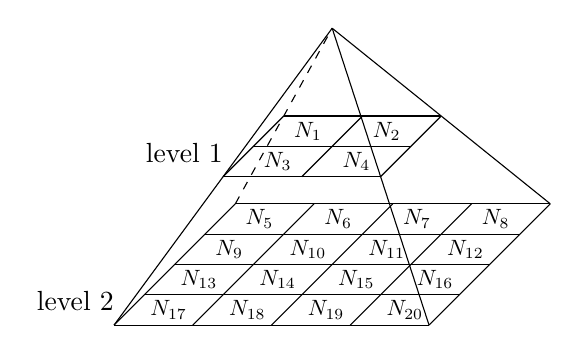
\begin{tikzpicture}
            % level 1
            \node at (-1.8, 1.5, 0.2) {level 1};
            \foreach \x [count=\xi] in {-0.5, 0.5}{
                \foreach \z [count=\zi] in {-0.5, 0.5}{
                    \pgfmathtruncatemacro{\i}{\zi*2 + \xi - 2}
                    \node[scale=0.8] at(\x, 1.5, \z) {$N_{\i}$};
                }
            }
            \foreach \x in {-1,...,1}{\draw (\x,1.5,-1) -- (\x,1.5,1);}
            \foreach \z in {-1,...,1}{\draw (-1,1.5,\z) -- (1,1.5,\z);}
            % level 2
            \node at (-2.8, 0, 1.2) {level 2};
            \foreach \x [count=\xi] in {-1.5,-0.5,...,1.5}{
                \foreach \z [count=\zi] in {-1.5,-0.5,...,1.5}{
                    \pgfmathtruncatemacro{\i}{\zi*4 + \xi}
                    \node[scale=0.8] at(\x, 0, \z) {$N_{\i}$};
                }
            }
            \foreach \x in {-2,...,2}{\draw (\x,0,-2) -- (\x,0,2);}
            \foreach \z in {-2,...,2}{\draw (-2,0,\z) -- (2,0,\z);}
            % pyramid
            \draw (-2,0,2) -- (0,3,0);
            \draw (2,0,2) -- (0,3,0);
            \draw (2,0,-2) -- (0,3,0);
            \draw[dashed] (-2,0,-2) -- (0,3,0);
        \end{tikzpicture}
    }
\end{minipage}\quad%
\begin{minipage}[t]{.33\linewidth}
    \resizebox{\linewidth}{!}{%
        \begin{tikzpicture}
            \node[scale=1.5] at (0, 2.5) {level 2};
            \foreach \x in {-2,...,2}{\draw (\x,-2) -- (\x,2);}
            \foreach \y in {-2,...,2}{\draw (-2,\y) -- (2,\y);}
            \foreach \y [count=\yi] in {1.5,0.5,...,-1.5}{%
                \foreach \x [count=\xi] in {-1.5,-0.5,...,1.5}{%
                    \pgfmathtruncatemacro{\i}{\yi*4 + \xi - 4}
                    \node [circle,fill,inner sep=1.2pt] at (\x,\y) {};
                    \ifthenelse{\i=10 \OR \i=11 \OR \i=12 \OR \i=14 \OR \i=15 \OR \i=16}{
                        \node[scale=1.2] at (\x+0.25,\y-0.25) {\contour{white}{$o_{\i}$}};
                    }{
                        \node[scale=1.2] at (\x+0.25,\y-0.25) {$o_{\i}$};
                    }
                }
            }
            \draw[red,rounded corners,thick] (-0.9,-2.1) rectangle (2.1,0.9);
            \node[red,scale=1.5] at (-1,-2.2) {$\alpha$};
            \node[red,scale=1.5] at (2.2,1) {$\beta$};
            \begin{pgfonlayer}{background}
                \fill[color=black!20] (-1,0) rectangle (2,1);
                \fill[pattern=north east lines,pattern color=blue!70] (-1,-2) rectangle (2,0);
            \end{pgfonlayer}
        \end{tikzpicture}
    }
\end{minipage}
}
    \caption{Data and Grid Partition}\label{fig:access-control:access-tree-struct}
  \end{subfigure}
  \begin{subfigure}[b]{\linewidth}
    \centering
    \resizebox{.7\linewidth}{!}{\begin{tikzpicture}
    \tikzstyle{tree node}=[
        rectangle split,
        rectangle split horizontal,
        rectangle split ignore empty parts,
        draw
    ]
    \tikzstyle{tree}=[
        every node/.style={tree node},
        edge from parent path={},
        level/.style={level distance=1cm},
        level 2/.style={sibling distance=4cm},
        level 3/.style={sibling distance=1cm},
    ]

    \path[tree] node (root) {$N_0$}
    child {
        node (l1) {
            \nodepart{one} $N_1$ \nodepart{two} $N_2$
            \nodepart{three} $N_3$ \nodepart{four} \contour{white}{$N_4$}
        }
        child {
            node (l21) {
                \nodepart{one} $N_{5}$ \nodepart{two} $N_{6}$
                \nodepart{three} $N_{9}$ \nodepart{four} $N_{10}$
            }
            child {node (o1) {$o_1$}}
            child {node (o2) {$o_2$}}
            child {node (o5) {$o_5$}}
            child {node [fill=black!20, text=black] (o6) {$o_6$}}
        }
        child {
            node (l22) {
                \nodepart{one} $N_{7}$ \nodepart{two} $N_{8}$
                \nodepart{three} $N_{11}$ \nodepart{four} $N_{12}$
            }
            child {node (o3) {$o_3$}}
            child {node (o4) {$o_4$}}
            child {node (o7) [fill=black!20, text=black] {$o_7$}}
            child {node (o8) [fill=black!20, text=black] {$o_8$}}
        }
        child {
            node (l23) {
                \nodepart{one} $N_{13}$ \nodepart{two} \contour{white}{$N_{14}$}
                \nodepart{three} $N_{17}$ \nodepart{four} \contour{white}{$N_{18}$}
            }
            child {node (o9) {$o_9$}}
            child {node (o10) {$o_{10}$}}
            child {node (o13) {$o_{13}$}}
            child {node (o14) {$o_{14}$}}
        }
        child {
            node (l24) {
                \nodepart{one} $N_{15}$ \nodepart{two} $N_{16}$
                \nodepart{three} $N_{19}$ \nodepart{four} $N_{20}$
            }
            child {node (o11) {$o_{11}$}}
            child {node (o12) {$o_{12}$}}
            child {node (o15) {$o_{15}$}}
            child {node (o16) {$o_{16}$}}
        }
    };

    \begin{pgfonlayer}{background}
        \fill[pattern=north east lines,pattern color=blue!70] (l1.three split north) rectangle (l1.south east);
        \fill[pattern=north east lines,pattern color=blue!70] (l23.one split north) rectangle (l23.two split south);
        \fill[pattern=north east lines,pattern color=blue!70] (l23.three split north) rectangle (l23.south east);
    \end{pgfonlayer}

    \foreach \a/\b in {
        root.south/l1,
        l1.one south/l21,
        l1.two south/l22,
        l1.three south/l23,
        l1.four south/l24,
        l21.one south/o1,
        l21.two south/o2,
        l21.three south/o5,
        l21.four south/o6,
        l22.one south/o3,
        l22.two south/o4,
        l22.three south/o7,
        l22.four south/o8,
        l23.one south/o9,
        l23.two south/o10,
        l23.three south/o13,
        l23.four south/o14,
        l24.one south/o11,
        l24.two south/o12,
        l24.three south/o15,
        l24.four south/o16%
    }
    \draw [style=edge from parent] (\a) -- (\b.north);

    \node[tree node,right=0.8cm of root] (data)
    {$gb_0$ \nodepart{two} $\Upsilon_0$ \nodepart{three} $sig_0$};

    \draw[dashed,-latex] (data) -- (root);

    \begin{customlegend}[
        legend cell align=left,
        legend image code/.code={%
            \draw[#1] (0cm,-0.15cm) rectangle (0.3cm,0.15cm);
        },
        legend style={draw=none,left=2cm of root,yshift=-0.3cm,font={\Large}}
    ]
        \addlegendimage{black,fill=black!20}
        \addlegendentry{APP signature}
        \addlegendimage{black,pattern=north east lines,pattern color=blue!70}
        \addlegendentry{APS signature}
    \end{customlegend}
\end{tikzpicture}
}
    \caption{Index}\label{fig:access-control:access-tree-index}
  \end{subfigure}
  \caption{Access-Policy-Preserving Grid-Tree (AP$^2$G-Tree)}\label{fig:access-control:access-tree}
\end{figure}

Consider a 2D data space for illustration. \Cref{fig:access-control:access-tree-struct} shows a multi-layer grid system, which partitions the query attribute space recursively into multiple levels of grid cells until each cell contains only one record. The bounding box of each cell is called a grid box. \Cref{fig:access-control:access-tree-index} shows the corresponding AP$^2$G-tree for the records in \cref{fig:access-control:access-tree-struct}. Each grid cell has a corresponding tree node $N_i$ in the AP$^2$G-tree, which consists of three components: grid box\footnote{A grid box is represented by the coordinates of its lower-left and upper-right points.} (denoted by $gb_i$), access policy ($p_i$), and APP signature (denoted by $sig_i$). The latter two components are computed from its $C$ child entries, $c_1, \dots, c_C$, in the following fashion.

\begin{definition}[AP$^2$G-tree Non-Leaf Node]
  Let ${sk}_{\textrm{DO}}$ be the signing key of the DO and $H(\cdot)$ a cryptographic hash function. The access policy and APP signature of a non-leaf node are defined as:
  \begin{align*}
    p_i   & = p_{c_1}  \lor  p_{c_2}  \lor  \dots  \lor  p_{c_C} \\
    sig_i & = \textsf{ABS.Sign}({sk}_{\textrm{DO}}, gb_i , p_i)
  \end{align*}
\end{definition}
For example, in \cref{fig:access-control:access-tree-index}, the access policy for $N_1$ is computed as $p_{N_1} = p_{N_5} \lor p_{N_6} \lor p_{N_9} \lor p_{N_{10}}$, and its APP signature is $sig_{N_1} = \textsf{ABS.Sign}({sk}_{\textrm{DO}}$, $gb_{N_1}$, $p_{N_1})$.

\begin{definition}[AP$^2$G-tree Leaf Node]
  The access policy and APP signature of a leaf node are identical to those of the single record lying in the corresponding cell.
\end{definition}
For example, for leaf node $N_5$, its policy and signature are $\Upsilon_{o_1}$ and $\sigma_{o_1}$, respectively.

The AP$^2$G-tree is built by the DO in a bottom-up fashion and is then outsourced to the SP\@.
It is worth noting that the AP$^2$G-tree is always a full tree, since we treat data records not existing in the original database as pseudo records inaccessible to any client, as explained in \cref{sec:access-control:equality-query}. This construction yields a space cost of $O((n + \log(n))m)$, where $n$ is the size of the index space and $m$ is the size of the monotone span program of the access policies. With the definitions above, the access policy of a non-leaf node essentially represents whether or not a client can access any record inside the grid box of this node. This property will allow us to perform effective pruning in the construction of VO during query processing.

On the SP side, the processing of a range query $[\alpha,\beta]$ can be executed as a breadth-first search. Starting from the root node, if a non-leaf node partially intersects the query range, it will be branched, i.e., its subtree is further explored. On the other hand, if a non-leaf node is fully covered by the query range, the SP will check whether or not the query client is allowed to access this node. If access is prohibited, the SP will run \textsf{ABS.Relax} to compute the APS signature for this node and add this signature to the VO\@. In contrast, if the access is permitted, the SP will further explore the subtree until a leaf node is reached. The process of handling a leaf node is the same as that for an equality query. Finally, similar to an equality query, all the results, as well as the VO, will be encrypted using AES and CP-ABE before they are transmitted to the client.

To establish the soundness and completeness of the query results, the client checks the VO in two aspects:
\begin{itemize}
  \item \textbf{Soundness check}. All of the signatures in the VO are valid; for an inaccessible node, the predicate of the corresponding signature is indeed $\lor_{a \in \mathbb{A}\backslash\mathcal{A}} a$; for an accessible record, it is indeed inside the query range $[\alpha, \beta]$.
  \item \textbf{Completeness check}. The union of the indexing spaces for each entry of the VO covers the whole query range $[\alpha, \beta]$. Note that this check is sufficient because one and only one entry is expected for each indexing space.
\end{itemize}

\begin{algorithm}[thp]
  \caption{Authentication of Range Queries}\label{alg:access-control:range-query}
  \SetKwBlock{DO}{ADS Generation (by the DO)}{}
  \SetKwBlock{SP}{VO Construction (by the SP)}{}
  \SetKwBlock{Client}{Result Verification (by the client)}{}
  \SetKw{forin}{in}
  \SetKw{is}{is}
  \DO{%
    \For{each data record $\langle o_i, v_i, \Upsilon_i\rangle$}{%
      $\sigma_i \gets \textsf{ABS.Sign}({sk}_{\textrm{DO}}, H(o_i) | H(v_i) , \Upsilon_i)$\;
    }
    \For{$gb_i$ \forin~each \textnormal{AP$^2$G-tree} non-leaf node}{%
      $p_i \gets \lor_{k=1}^C p_{c_k}$\;
      $sig_i \gets \textsf{ABS.Sign}({sk}_{\textrm{DO}}, H(gb_i), p_i)$\;
    }
    Outsource all $\langle o_i, v_i, \Upsilon_i, \sigma_i\rangle$ and $\langle gb_i, p_i, sig_i\rangle$ to SP\;
  }
  \SP{%
    \KwIn{Query range $[\alpha, \beta]$, access role set $\mathcal{A}$}
    create an empty queue $q$\;
    $q$.enqueue(AP$^2$G-tree root)\; % chktex 36
    \While{$q$ \textnormal{{is not empty}}}{%
      $n$ $\gets$ $q$.dequeue()\; % chktex 36
      \lIf{$n$ partially intersects $[\alpha, \beta]$}{%
        $q$.enqueue($n$.children)% chktex 36
      }
      \ElseIf{$n$ lies inside $[\alpha, \beta]$}{%
        \eIf{$n$ is accessible to the client}{%
          \lIf{n~\is~a leaf node}{%
            add$\langle o_n, v_n, \sigma_n, \Upsilon_n\rangle$to VO%
          }
          \lElse{%
            $q$.enqueue($n$.children)% chktex 36
          }
          }{%
          \eIf{n~\is~a leaf node}{%
            $\hat{\sigma}_{n,\mathcal{A}} \gets \textsf{ABS.Relax}(\sigma_n, \mathbb{A}\backslash\mathcal{A})$\;
            add $\langle H(v_n), \hat{\sigma}_{n,\mathcal{A}}\rangle$ to VO\; % chktex 36
            }{%
            $\hat{sig}_{n,\mathcal{A}} \gets \textsf{ABS.Relax}(sig_n, \mathbb{A}\backslash\mathcal{A})$\;
            add $\langle gb_n, \hat{sig}_{n,\mathcal{A}}\rangle$ to VO\;
          }
        }
      }
    }
    send $\textsf{CP-ABE.Encrypt}(pp, VO, \land_{a \in \mathcal{A}} a)$ to the client;
  }
  \Client{%
    run \textsf{CP-ABE.Decrypt} to decrypt the VO\;
    check if the union of the region for each entry in the VO covers $[\alpha, \beta]$\;
    $\hat{\Upsilon}_{\mathcal{A}} \gets \lor_{a \in \mathbb{A}\backslash\mathcal{A}} a$\;
    \For{each entry $e$~\forin~VO}{%
      \uIf{$e$ is accessible to the client}{%
        check $o_e \in [\alpha, \beta]$ and $\Upsilon_e(\mathcal{A}) = 1$\;
        run \textsf{ABS.Verify}$(mvk, H(o_e)|H(v_e), \Upsilon_e, \sigma_e)$\;
      }
      \uElseIf{e~\is~a data record}{%
        run \textsf{ABS.Verify}$(mvk, H(o_e)|H(v_e), \hat{\Upsilon}_{\mathcal{A}}, \hat{\sigma}_{e,\mathcal{A}})$\;
      }
      \lElse{
        run \textsf{ABS.Verify}$(mvk, gb_e, \hat{\Upsilon}_{\mathcal{A}}, \hat{sig}_{e,\mathcal{A}})$%
      }
    }
  }
\end{algorithm}

We summarize the algorithm for authenticating range queries with the zero-knowledge confidentiality in \cref{alg:access-control:range-query}.
\Cref{fig:access-control:access-tree} illustrates an example in which the client can only access $o_6, o_7, o_8$ (highlighted with a gray color) in the range query $[\alpha,\beta]$ (highlighted as the red rectangle in \cref{fig:access-control:access-tree-struct}). As a result, the SP will return the records $o_6$, $o_7$ and $o_8$, as well as their APP signatures, to the client. Moreover, the SP will run the \textsf{ABS.Relax} algorithm with the APP signatures of $N_4$, $N_{14}$ and $N_{18}$ as inputs. The derived APS signatures will be sent to the client as part of the VO, to prove their inaccessibility. During result verification, the client will check whether or not all of the signatures in the VO are valid (to verify the soundness) and whether or not the query range $[\alpha, \beta]$ is indeed covered by the union of the indexing spaces for $N_4$, $N_{14}$, $N_{18}$, $o_6$, $o_7$, and $o_8$ (to verify the completeness).

\subsection{Join Query Authentication}

\begin{figure}[t]
  \centering
  \resizebox{.75\linewidth}{!}{\begin{tikzpicture}
    \tikzstyle{tree node}=[
        rectangle split,
        rectangle split horizontal,
        rectangle split ignore empty parts,
        draw
    ]
    \tikzstyle{tree}=[
        every node/.style={tree node},
        edge from parent path={},
        level/.style={level distance=0.8cm},
        level 2/.style={sibling distance=3cm},
        level 3/.style={sibling distance=2cm},
    ]
    \tikzstyle{diagonal fill}=[
            path picture={
                \fill[#1] (path picture bounding box.north west) |-
                          (path picture bounding box.south east) -- cycle;
            }
    ]

    \path[tree] node (r_root) {$R_0$}
    child {
        node (r_l1) {
            \nodepart{one} $R_1$ \nodepart{two} \contour{white}{$R_2$}
        }
        child {
            node (r_l21) {
                \nodepart{one} $R_{3}$ \nodepart{two} $R_{4}$
            }
            child {node (r1) [fill=black!20, text=black] {$r_1$}}
            child {node (r2) [diagonal fill=black!30, text=black] {$r_2$}}
        }
        child {
            node (r_l22) {
                \nodepart{one} $R_{5}$ \nodepart{two} $R_{6}$
            }
            child {node (r3) {$r_3$}}
            child {node (r4) {$r_4$}}
        }
    };

    \path[tree, grow=up] node[below=5.1cm of r_root] (s_root) {$S_0$}
    child {
        node (s_l1) {
        \nodepart{one} $S_1$ \nodepart{two} $S_2$
        }
        child {
            node (s_l22) {
                \nodepart{one} $S_{5}$ \nodepart{two} $S_{6}$
            }
            child {node (s4) {$s_4$}}
            child {node (s3) [diagonal fill=black!30, text=black] {$s_3$}}
        }
        child {
            node (s_l21) {
                \nodepart{one} $S_{3}$ \nodepart{two} \contour{white}{$S_{4}$}
            }
            child {node (s2) {$s_2$}}
            child {node (s1) [fill=black!20, text=black] {$s_1$}}
        }
    };

    \begin{pgfonlayer}{background}
        \fill[pattern=north east lines,pattern color=blue!70] (r_l1.one split north) rectangle (r_l1.south east);
        \fill[pattern=north east lines,pattern color=blue!70] (s_l21.one split north) rectangle (s_l21.south east);
    \end{pgfonlayer}

    \foreach \a/\b in {
        r_root.south/r_l1,
        r_l1.one south/r_l21,
        r_l1.two south/r_l22,
        r_l21.one south/r1,
        r_l21.two south/r2,
        r_l22.one south/r3,
        r_l22.two south/r4%
    }
    \draw [style=edge from parent] (\a) -- (\b.north);
    \foreach \a/\b in {
        s_root.north/s_l1,
        s_l1.one north/s_l21,
        s_l1.two north/s_l22,
        s_l21.one north/s1,
        s_l21.two north/s2,
        s_l22.one north/s3,
        s_l22.two north/s4%
    }
    \draw [style=edge from parent] (\a) -- (\b.south);

    \coordinate (mid) at ($(r_root)!.5!(s_root)$);

    \draw[thick] ($(mid) + (-3.3cm,0.1cm)$) rectangle
                 ($(mid) + (3.3cm,3.3cm)$) node[anchor=north east,scale=1] {Table $R$};

    \draw[thick] ($(mid) + (-3.3cm,-0.1cm)$) rectangle
                 ($(mid) + (3.3cm,-3.3cm)$) node[anchor=south east,scale=1] {Table $S$};

    \draw[red, rounded corners, thick]
        ($(mid) - (2.9cm,0.85cm)$) rectangle ($(mid) + (2.9cm,0.85cm)$);
    \node[red,scale=1.2] at ($(mid) + (-3.1cm,0.25cm)$) {$\alpha$};
    \node[red,scale=1.2] at ($(mid) + ( 3.1cm,0.25cm)$) {$\beta$};

    \begin{customlegend}[
        legend cell align=left,
        rectangle legend/.style={
            legend image code/.code={%
                \draw[black,#1] (0cm,-0.15cm) rectangle (0.3cm,0.15cm);
            }
        },
        rectangle legend multiline/.style={
            legend image code/.code={%
                \draw[black,#1] (0cm,-0.15cm) rectangle (0.3cm,0.15cm);
            }
        },
        legend style={
            draw=none,
            cells={align=left},
            above left=1.5cm and 3.5cm of mid
        }
    ]
        \addlegendimage{rectangle legend={fill=black!20}}
        \addlegendentry{APP signature}
        \addlegendimage{rectangle legend={pattern=north east lines,pattern color=blue!70}}
        \addlegendentry{APS signature}
        \addlegendimage{rectangle legend multiline={diagonal fill=black!30}}
        \addlegendentry{Non-result accessible record}
    \end{customlegend}
\end{tikzpicture}
}
  \caption{Join Query Authentication}\label{fig:access-control:join}
\end{figure}

\begin{algorithm}[t]
  \caption{Authentication of Joins (VO Construction)}\label{alg:access-control:join-query}
  \SetKw{forin}{in}
  \SetKw{is}{is}
  \KwIn{AP$^2$G-tree $\mathcal{T}_R, \mathcal{T}_S$, Query range $[\alpha, \beta]$, access role set $\mathcal{A}$}
  create an empty queue $q$\;
  $q$.enqueue($\langle \mathcal{T}_R$ root, $\mathcal{T}_S$ root$\rangle$)\; % chktex 36
  \While{$q$ \textnormal{{is not empty}}}{%
    $\langle n_R, n_S\rangle$ $\gets$ $q$.dequeue()\; % chktex 36
    \uIf{$n_R$ partially intersects $[\alpha, \beta]$}{%
      \lFor{$n$~\forin~$n_R$.children}{%
        $q$.enqueue($\langle n, n_S\rangle$)% chktex 36
      }
    }
    \ElseIf{$n_R$ lies inside $[\alpha, \beta]$}{%
      \uIf{$n_R$ is accessible to the client}{%
        $n_S \gets$ the smallest node under $n_S$, which also covers the region of $n_R$\;
        \uIf{$n_S$ is accessible to the client}{%
          \eIf{$n_R$~\is~a leaf node}{%
            \tcp{In this case, $n_S$ is also a leaf node.}
            add APP signatures of $n_R$ and $n_S$ to VO\;
            }{%
            \lFor{$n$~\forin~$n_R$.children}{%
              $q$.enqueue($\langle n, n_S\rangle$)% chktex 36
            }
          }

        }
        \lElse{%
          compute and add APS signature of $n_S$ to VO%
        }
      }
      \lElse{%
        compute and add APS signature of $n_R$ to VO%
      }
    }
  }
  send $\textsf{CP-ABE.Encrypt}(pp, VO, \land_{a \in \mathcal{A}} a)$ to the client\;
\end{algorithm}


Next, we discuss how to extend the range query authentication algorithm to support join queries. Consider an equi-join query over two tables $R$ and $S$, $R \Join_{R.o = S.o} S \land R.o \in [\alpha, \beta]$, with client's access role set $\mathcal{A}$. The SP should return all record pairs in the query range that are accessible to the query client and satisfy the join condition.
For example, in \cref{fig:access-control:join}, the client can access $r_1$, $r_2$ from $R$ and $s_1$, $s_3$ from $S$ (highlighted with a gray color); the join result will be the pair of records $\langle r_1, s_1\rangle$.

To process the join query, the SP starts by executing a breadth-first search from the root node of the AP$^2$G-tree for the table $R$. The tree search algorithm is almost identical to the one in the range query processing, except for two aspects. First, if a node for $R$, denoted as $N_R$, is accessible to the client, the SP will first check whether or not there exists an inaccessible node in the AP$^2$G-tree for the table $S$ that covers $N_R$. If such a node, denoted as $N_S$, is found, $N_R$ cannot be part of the join result. Hence, the corresponding APS signature for $N_S$ is computed and appended to the VO\@. Otherwise, the subtree of $N_R$ is further explored. Second, an accessible record in $R$ is part of the result only if the matching record in $S$ is also accessible. In this case, the APP signatures for this pair of records will be appended to the VO\@. The rest of the algorithm is the same as the one in the range query processing.

We summarize the VO construction procedure in \cref{alg:access-control:join-query}, while the ADS generation and result verification procedures are the same as the ones in \cref{alg:access-control:range-query}.
In the example of \cref{fig:access-control:join}, the SP will return the records $r_1$ and $s_1$, as well as their APP signatures, to the client. Moreover, for the inaccessible nodes $R_2$ and $S_4$, their derived APS signatures will be returned as part of the VO\@. On the client side, to verify the soundness, the client will authenticate all the signatures in the VO and check whether or not $r_1$ and $s_1$ share the same value on the join attribute; to verify the completeness, the client will check whether or not the union of the indexing spaces for $R_2$, $S_4$, and $r_1$/$r_2$ covers the whole query range $[\alpha,\beta]$.

This solution can be easily extended to support more general join queries, such as multi-way join and inequality join. The general idea is similar, i.e., using the APS signature of an inaccessible record/node to prove that a certain space does not contribute to the join result. The client verifies the soundness by the given results and their associated APP signatures, and verifies the completeness by checking whether or not the result set and the space represented by the APS signatures together cover the whole query range.

\section{Security Analysis}\label{sec:access-control:security-analysis}

In this section, we perform a security analysis on our proposed ABS scheme and query authentication algorithms.

\subsection{Security Analysis on ABS}\label{sec:access-control:security-analysis-abs}

In order to facilitate our security analysis, we first present the formal definitions of our security notions.

\begin{definition}[Perfect Privacy]\label{def:access-control:abs-privacy}
  We say an ABS scheme achieves perfect privacy if for all $(msk$, $mvk) \gets \textsf{ABS.Setup}(1^\lambda)$, all messages $m$, such that:
  \begin{itemize}
    \item For all attribute sets $\mathcal{A}_1$, $\mathcal{A}_2$, all signing keys ${sk}_{\mathcal{A}_1} \gets \textsf{ABS.KeyGen}(msk, \mathcal{A}_1)$, ${sk}_{\mathcal{A}_2} \gets \textsf{ABS.KeyGen}(msk, \mathcal{A}_2)$, all claim-predicates $\Upsilon$ such that $\Upsilon(\mathcal{A}_1)=\Upsilon(\mathcal{A}_2)=1$, the distributions of $\textsf{ABS.Sign}({sk}_{\mathcal{A}_1}$, $m$, $\Upsilon)$ and $\textsf{ABS.Sign}({sk}_{\mathcal{A}_2}$, $m$, $\Upsilon)$ are identical.
    \item For all attribute sets $\mathcal{A}, \mathcal{A}'$, all signing keys ${sk}_{\mathcal{A}} \gets \textsf{ABS.KeyGen}(msk$, $\mathcal{A})$, ${sk}_{\mathcal{A}'} \gets \textsf{ABS.KeyGen}(msk$, $\mathcal{A}')$, all claim-predicates $\Upsilon$ such that $\Upsilon(\mathbb{A}\backslash\mathcal{A}') = 0$ and all signatures $\sigma_{m, \Upsilon} \gets \textsf{ABS.Sign}({sk}_{\mathcal{A}}$, $m$, $\Upsilon)$, the distributions of \textsf{ABS.Sign}$(sk_{\mathcal{A}'}$, $m$, $\lor_{a \in \mathcal{A}'} a)$ and \textsf{ABS.Relax}$(\sigma_{m, \Upsilon}$, $\mathcal{A}')$ are identical.
  \end{itemize}
\end{definition}
This property ensures that an ABS signature generated by \textsf{ABS.Sign} or \textsf{ABS.Relax} will not leak the information about which set of attributes or signing key was used in signing. This is a necessary condition to support zero-knowledge.

\begin{definition}[Unforgeability]\label{def:access-control:abs-unf}
  We say an ABS scheme is unforgeable if the success probability of any polynomial-time adversary is negligible in the following experiment:
  \begin{itemize}
    \item Run $(msk, mvk) \gets \textsf{ABS.Setup}(1^\lambda)$ and give $mvk$ to the adversary.
    \item The adversary is given access to oracle $\textsf{ABS.Sign}(\cdot)$, which, on input $(m, \Upsilon)$, outputs the corresponding signature $\sigma$.
      Let ${\{m^{(\iota)}, \Upsilon^{(\iota)}, \sigma^{(\iota)}\}}_{\iota=1}^q$ be the message-policy-signature tuples obtained by the adversary with its $q$ queries.
    \item At the end the adversary outputs $(m^*, \Upsilon^*, \sigma^*)$.
  \end{itemize}
  We say the adversary succeeds if $\textsf{ABS.Verify}(mvk$, $m^*$, $\Upsilon^*$, $\sigma^*)$ outputs 1 and one of the following results is true:
  \begin{itemize}
    \item $m^\ast \neq m^{(\iota)}$ for $\iota=1$ to $q$.
    \item For each $\iota$ such that $m^\ast = m^{(\iota)}$, $\Upsilon^\ast$ is a more restricted policy compared with $\Upsilon^{(\iota)}$. Furthermore, $\Upsilon^\ast$ is of the form
      $(\lor_{a \in \mathcal{A}'} a)$ for some $\mathcal{A'} \subset \mathbb{A}$, where $\mathbb{A}$ represents the attribute universe.
  \end{itemize}
\end{definition}
This property ensures that a malicious SP could convince the client of an incorrect answer with at most a negligible probability.
It is worth noting that this security model of ABS is defined with respect to the threat model of our problem. And it is weaker than the typical security model for ABS in two ways. First, the attacker will not have access to signing keys for different attributes, since the DO is the only party who processes them. Second, a valid forgery must be either a signature on a new message or on a message that has been signed on a more restricted policy. By contrast, in a typical security model of ABS, any new message-policy pair is considered a valid forgery.

Now we reach the theorem on the security of our ABS scheme.

\begin{restatable}{theorem}{abssecuritytheorem}\label{thm:access-control:abs-sec}
  The construction of \cref{sec:access-control:abs} satisfies the security properties of Perfect Privacy (\cref{def:access-control:abs-privacy}) and Unforgeability (\cref{def:access-control:abs-unf}) in the generic group model.
\end{restatable}

\begin{proof}
  Please see \cref{app:access-control-abs-sec} for detailed proofs.
\end{proof}

\subsection{Security Analysis on Query Authentication}\label{sec:access-control:security-analysis-query}

The formal definition for desired security on our query authentication algorithms consists of two properties, namely unforgeability and zero-knowledge.

\begin{definition}[Unforgeability]\label{def:access-control:query-secure}
  We say our proposed query authentication algorithms are unforgeable if the success probability of any polynomial-time adversary is negligible in the following experiment:
  \begin{itemize}
    \item Run the ADS generation and give all $\langle o_i$, $v_i$, $\Upsilon_i$, $\sigma_i\rangle$ and $\langle gb_i$, $p_i$, $sig_i\rangle$ to the adversary.
    \item The adversary outputs a query $q$ (either a range or join query), an access role set $\mathcal{A}$, a result set $RS$, and a VO\@.
  \end{itemize}
  We say the adversary succeeds if the VO passes the result verification and one of the following results is true:
  \begin{itemize}
    \item The result set $RS$ contains a record $\langle o^*, v^*, \Upsilon^*\rangle$, such that $\langle o^*, v^*, \Upsilon^*\rangle$ $\neq$ $\langle o_i, v_i, \Upsilon_i\rangle$, $\forall i$.
    \item The result set $RS$ contains a record $\langle o^*, v^*, \Upsilon^*\rangle$, such that $o^*$ does not satisfy the query $q$ or $\Upsilon^*(\mathcal{A}) = 0$.
    \item There exists a record $\langle o_j, v_j, \Upsilon_j\rangle$ not in $RS$, such that $j \in \{i\}$, $o_j$ satisfies the query $q$, and $\Upsilon_j(\mathcal{A})= 1$.
  \end{itemize}
\end{definition}

This property ensures that a malicious SP could convince the client of an incorrect or incomplete answer with at most a negligible probability.

\begin{definition}[Zero-Knowledge]\label{def:access-control:query-zero-knowledge}
  We say our proposed query authentication algorithms are zero-knowledge if the success probability of any polynomial-time adversary is negligible in the following experiment:
  \begin{itemize}
    \item \textbf{Game Real}:
      \begin{itemize}
        \item Setup: the adversary picks a database $\mathcal{D}$ and an access role set $\mathcal{A}$, the real challenger runs ADS generation over this database.
        \item Query: the adversary runs the interactive query protocol with the challenger under the access role set $\mathcal{A}$.
      \end{itemize}
    \item \textbf{Game Ideal}:
      \begin{itemize}
        \item Setup: the adversary picks a database $\mathcal{D} = \{\langle o_i, v_i, \Upsilon_i\rangle\}$ and an access role set $\mathcal{A}$, the simulator runs ADS generation over a database $\mathcal{D}'= \{\langle o'_i, v'_i, \Upsilon'_i\rangle\}$, such that:
        \begin{align*}
          \langle o'_i, v'_i, \Upsilon'_i\rangle &= \left\{%
          \begin{array}{ll}
          \langle o_i, v_i, \Upsilon_i \rangle & \text{if }\Upsilon_i(\mathcal{A}) = 1, \\
          \langle o_i, \textsf{random}, {Role}_{\emptyset}\rangle & \text{otherwise.}
          \end{array}%
          \right.%
        \end{align*}
        \item Query: the adversary runs the interactive query protocol with the simulator under the access role set $\mathcal{A}$.
      \end{itemize}
  \end{itemize}
  We say the adversary succeeds if he/she can distinguish the above two games.
\end{definition}

This property ensures that a malicious client could extract any information regarding the database beyond accessible records with at most a negligible probability. It is worth noting that, by achieving the zero-knowledge confidentiality, the data content confidentiality and access policy confidentiality are automatically guaranteed.

With the above security definitions, we can show that our proposed query authentication algorithms indeed satisfy the desired security requirements.

\begin{restatable}{theorem}{querysecuritytheorem}\label{thm:access-control:sec}
  Our proposed query authentication algorithms satisfy the security properties of Unforgeability (\cref{def:access-control:query-secure}) and Zero-Knowledge (\cref{def:access-control:query-zero-knowledge}).
\end{restatable}

\begin{proof}
  Please see \cref{app:access-control-sec} for detailed proofs.
\end{proof}

\section{Optimizations}\label{sec:access-control:opt}

This section presents two optimization techniques. They are orthogonal to each other, and therefore can be combined to maximize the performance.

\subsection{Hierarchical Role Assignment}
Since the performance of ABS depends on the number of input roles, one way to optimize the performance is to reduce the size of inaccessible predicates for query clients. Thus, we propose hierarchical role assignment. In a hierarchical structure, not possessing one access role implies the lack of some other access roles. For example, if the access role universe is $\{{Role}_A$, ${Role}_{A,S}$, ${Role}_{A,P}$, ${Role}_B$, ${Role}_{B,S}$, ${Role}_{B,P}\}$, which corresponds to a member of university $A$ or $B$, a student of university $A$ or $B$, and a professor of university $A$ or $B$, respectively. It is easy to see that a client who is not a member of university $A$ (access role ${Role}_A$) cannot have any access role associated with university $A$, i.e., ${Role}_{A,S}$ and ${Role}_{A,P}$. As such, the inaccessible predicate for a client with access role ${Role}_{B,S}$ can be simplified to ${Role}_A \lor {Role}_{B,P}$.

Regarding the performance, with hierarchical role assignment, the overhead of the DO setup time is expected to increase slightly, owing to a larger access policy in each record. For example, a record which can only be accessed by the professors of university $A$ will have the access policy ${Role}_{A} \land {Role}_{A,P}$, instead of just ${Role}_{A,P}$.
However, with a much smaller inaccessible predicate, the costs of the SP query time and client verification time can be reduced dramatically.

\subsection{Acceleration by Parallelism}
In our solution to range and join query authentication, the majority of computational overheads comes from the \textsf{ABS.Relax} operations. Fortunately, since these operations are independent to each other, they are highly parallelizable. In light of this, we can accelerate the authentication performance by embracing parallel computing architectures, such as multi-threading, GPU computing, and MapReduce. For example, when the SP processes a query, we can map all \textsf{ABS.Relax} jobs for the inaccessible nodes to the available computing units, whether they are CPU cores or worker nodes in the MapReduce model.

\section{Relaxing Zero-Knowledge Confidentiality Requirement}\label{sec:access-control:relaxing-zero-knowledge}

Zero-knowledge confidentiality is a strong requirement that may not be demanded in some less critical applications. In this section, we discuss how to boost the performance for range queries and join queries (\cref{sec:access-control:kd-tree}) and support more general continuous query attributes (\cref{sec:access-control:continuous-attribute}), when such a requirement is relaxed to the less restrictive access policy confidentiality.

\subsection{Using $k$-d Tree Index Structure}\label{sec:access-control:kd-tree}

\begin{algorithm}[t]
    \caption{AP$^2k$d-Tree Split}\label{alg:access-control:kd-split}
    \SetKwFunction{Split}{Split}
    \SetKw{forto}{to}
    \Fn{\Split{$\{\Upsilon_1, \dots, \Upsilon_n\}$}}{%
        \KwIn{Access Policies $\{\Upsilon_1, \dots \Upsilon_n\}$}
        \KwOut{Hyperplane~$x = \underset{x}{\arg\min}\,f(\Upsilon_1 \lor \dots \lor \Upsilon_x, \Upsilon_{x+1} \lor \dots \lor \Upsilon_n)$}
        \For{$i = 1~\forto~n$}{%
            convert $\Upsilon_i$ to DNF, i.e., $\Upsilon_i = \lor_{A_j \in X_i} \land_{a_{ij} \in A_j} a_{ij}$\;
        }
        \lIf{$n = 2$}{$x \gets 1$}
        \uElseIf{$n = 3$}{\leIf{$|X_1 \cap X_2| < |X_2 \cap X_3|$}{$x \gets 1$}{$x \gets 2$}}
        \Else{%
            $x' \gets $\Split{$\{\Upsilon_1, \dots, \Upsilon_{n-1}\}$}\;
            $a \gets |(X_1 \cup \dots \cup X_{x'}) \cap (X_{x'+1} \cup \dots \cup X_{n-1})|$\;
            $b \gets |(X_{x'+1} \cup \dots \cup X_{n-1}) \cap X_n|$\;
            \leIf{$a < b$}{$x \gets x'$}{$x \gets n - 1$}
        }
        \Return{$x$}\;
    }
\end{algorithm}

Recall in \cref{sec:access-control:range-query} that the grid tree is chosen to prevent information leakage through the tree structure. However, it is well known that the grid tree is not the most efficient index structure, especially for sparse multi-dimensional databases. Here, in the system that only requires the access policy confidentiality, we propose \emph{access-policy-preserving $k$-d-tree} (AP$^2k$d-tree) as an alternative ADS that uses $k$-d tree~\cite{10.1145/361002.361007} to optimize the performance.

\begin{figure}[t]
    \centering
    \begin{subfigure}[b]{\linewidth}
        \centering
        \resizebox{.7\linewidth}{!}{\begin{minipage}[t]{.6\linewidth}
    \resizebox{\linewidth}{!}{%
        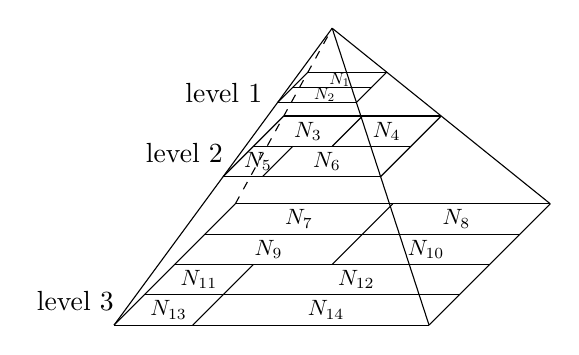
\begin{tikzpicture}
            % level 1
            \node at (-1.3, 2.25, 0.2) {level 1};
            \draw(-0.5,2.25,-0.5) -- (-0.5,2.25,0.5);
            \draw(-0.5,2.25,-0.5) -- (0.5,2.25,-0.5);
            \draw(0.5,2.25,-0.5) -- (0.5,2.25,0.5);
            \draw(-0.5,2.25,0.5) -- (0.5,2.25,0.5);
            \draw(-0.5,2.25,0) -- (0.5,2.25,0);
            \foreach \x/\z [count=\i] in
            {0/-0.25,0/0.25}{
                \node[scale=0.6] at(\x, 2.25, \z) {$N_{\i}$};
            }
            % level 2
            \node at (-1.8, 1.5, 0.2) {level 2};
            \draw (-1,1.5,-1) -- (-1,1.5,1);
            \draw (-1,1.5,-1) -- (1,1.5,-1);
            \draw (1,1.5,-1) -- (1,1.5,1);
            \draw (-1,1.5,1) -- (1,1.5,1);
            \draw (-1,1.5,0) -- (1,1.5,0);
            \draw (0,1.5,-1) -- (0,1.5,0);
            \draw (-0.5,1.5,0) -- (-0.5,1.5,1);
            \foreach \x/\z [count=\i from 3] in
            {-0.5/-0.5,0.5/-0.5,-0.75/0.5,0.125/0.5}{
                \node[scale=0.8] at(\x, 1.5, \z) {$N_{\i}$};
            }
            % level 3
            \node at (-2.8, 0, 1.2) {level 3};
            \draw (-2,0,-2) -- (-2,0,2);
            \draw (-2,0,-2) -- (2,0,-2);
            \draw (2,0,-2) -- (2,0,2);
            \draw (-2,0,2) -- (2,0,2);
            \draw (-2,0,0) -- (2,0,0);
            \draw (0,0,0) -- (0,0,-2);
            \draw (-1,0,0) -- (-1,0,2);
            \draw (-2,0,1) -- (2,0,1);
            \draw (-2,0,-1) -- (2,0,-1);
            \foreach \x/\z [count=\i from 7] in
            {-1/-1.5,1/-1.5,-1/-0.5,1/-0.5,-1.5/0.5,0.5/0.5,-1.5/1.5,0.5/1.5}{
                \node[scale=0.8] at(\x, 0, \z) {$N_{\i}$};
            }

            % pyramid
            \draw (-2,0,2) -- (0,3,0);
            \draw (2,0,2) -- (0,3,0);
            \draw (2,0,-2) -- (0,3,0);
            \draw[dashed] (-2,0,-2) -- (0,3,0);
        \end{tikzpicture}
    }
\end{minipage}\quad%
\begin{minipage}[t]{.33\linewidth}
    \resizebox{\linewidth}{!}{%
        \begin{tikzpicture}
            \node[scale=1.5] at (0, 2.5) {level 3};
            \draw (-2,-2) -- (-2,2);
            \draw (-2,-2) -- (2,-2);
            \draw (2,-2) -- (2,2);
            \draw (-2,2) -- (2,2);

            % level 1
            \draw (-2,0) -- (2,0);
            % level 2
            \draw (0,0) -- (0,2);
            \draw (-1,0) -- (-1,-2);
            % level 3
            \draw (-2,1) -- (2,1);
            \draw (-2,-1) -- (2,-1);

            \foreach \y [count=\yi] in {1.5,0.5,...,-1.5}{%
                \foreach \x [count=\xi] in {-1.5,-0.5,...,1.5}{%
                    \pgfmathtruncatemacro{\i}{\yi*4 + \xi - 4};
                    \node [circle,fill,inner sep=1.2pt] at (\x,\y) {};
                    \ifthenelse{\i=10 \OR \i=11 \OR \i=12 \OR \i=14 \OR \i=15 \OR \i=16}{
                        \node[scale=1.2] at (\x+0.25,\y-0.25) {\contour{white}{$o_{\i}$}};
                    }{
                        \node[scale=1.2] at (\x+0.25,\y-0.25) {$o_{\i}$};
                    }
                }
            }
            \draw[red,rounded corners,thick] (-0.9,-2.1) rectangle (2.1,0.9);
            \node[red,scale=1.5] at (-1,-2.2) {$\alpha$};
            \node[red,scale=1.5] at (2.2,1) {$\beta$};
            \begin{pgfonlayer}{background}
                \fill[color=black!20] (-1,0) rectangle (2,1);
                \fill[pattern=north east lines,pattern color=blue!70] (-1,-2) rectangle (2,0);
            \end{pgfonlayer}
        \end{tikzpicture}
    }
\end{minipage}
}
        \caption{Data and Space Partition}\label{fig:access-control:access-kd-tree-struct}
    \end{subfigure}
    \begin{subfigure}[b]{\linewidth}
        \centering
        \resizebox{.7\linewidth}{!}{\begin{tikzpicture}
    \tikzstyle{tree node}=[
        rectangle split,
        rectangle split horizontal,
        rectangle split ignore empty parts,
        draw
    ]
    \tikzstyle{tree}=[
        every node/.style={tree node},
        edge from parent path={},
        level/.style={level distance=1cm},
        level 2/.style={sibling distance=7.5cm},
        level 3/.style={sibling distance=4.3cm},
        level 4/.style={sibling distance=2.1cm},
        level 5/.style={sibling distance=1cm},
    ]

    \path[tree] node (root) {$N_0$}
    child {
        node (l1) {
            \nodepart{one} $N_1$ \nodepart{two} $N_2$
        }
        child {
            node (l21) {
                \nodepart{one} $N_{3}$ \nodepart{two} $N_{4}$
            }
            child {
                node (l31) {
                    \nodepart{one} $N_{7}$ \nodepart{two} $N_{9}$
                }
                child {
                    node (l41) {
                        \nodepart{one} $N_{15}$ \nodepart{two} $N_{16}$
                    }
                    child {node (o1) {$o_1$}}
                    child {node (o2) {$o_2$}}
                }
                child {
                    node (l42) {
                        \nodepart{one} $N_{19}$ \nodepart{two} $N_{20}$
                    }
                    child {node (o5) {$o_5$}}
                    child {node [fill=black!20, text=black] (o6) {$o_6$}}
                }
            }
            child {
                node (l32) {
                    \nodepart{one} $N_{8}$ \nodepart{two} $N_{10}$
                }
                child {
                    node (l43) {
                        \nodepart{one} $N_{17}$ \nodepart{two} $N_{18}$
                    }
                    child {node (o3) {$o_3$}}
                    child {node (o4) {$o_4$}}
                }
                child {
                    node (l44) {
                        \nodepart{one} $N_{21}$ \nodepart{two} $N_{22}$
                    }
                    child {node [fill=black!20, text=black] (o7) {$o_7$}}
                    child {node [fill=black!20, text=black] (o8) {$o_8$}}
                }
            }
        }
        child{
            node (l22) {
                \nodepart{one} $N_{5}$ \nodepart{two} \contour{white}{$N_{6}$}
            }
            child {
                node (l33) {
                    \nodepart{one} $N_{11}$ \nodepart{two} $N_{13}$
                }
                child [sibling distance=1cm] {
                    node (l45) {$N_{23}$}
                    child {node (o9) {$o_9$}}
                }
                child [sibling distance=1cm] {
                    node (l46) {$N_{27}$}
                    child {node (o13) {$o_{13}$}}
                }
            }
            child {
                node (l34) {
                    \nodepart{one} $N_{12}$ \nodepart{two} $N_{14}$
                }
                child [sibling distance=3cm] {
                    node (l47) {
                        \nodepart{one} $N_{24}$
                        \nodepart{two} $N_{25}$
                        \nodepart{three} $N_{26}$
                    }
                    child {node (o10) {$o_{10}$}}
                    child {node (o11) {$o_{11}$}}
                    child {node (o12) {$o_{12}$}}
                }
                child [sibling distance=3cm] {
                    node (l48) {
                        \nodepart{one} $N_{28}$
                        \nodepart{two} $N_{29}$
                        \nodepart{three} $N_{30}$
                    }
                    child {node (o14) {$o_{14}$}}
                    child {node (o15) {$o_{15}$}}
                    child {node (o16) {$o_{16}$}}
                }
            }
        }
    };

    \begin{pgfonlayer}{background}
        \fill[pattern=north east lines,pattern color=blue!70] (l22.one split north) rectangle (l22.two split south);
    \end{pgfonlayer}

    \foreach \a/\b in {
        root.south/l1,
        l1.one south/l21,
        l1.two south/l22,
        l21.one south/l31,
        l21.two south/l32,
        l22.one south/l33,
        l22.two south/l34,
        l31.one south/l41,
        l31.two south/l42,
        l32.one south/l43,
        l32.two south/l44,
        l33.one south/l45,
        l33.two south/l46,
        l34.one south/l47,
        l34.two south/l48,
        l41.one south/o1,
        l41.two south/o2,
        l42.one south/o5,
        l42.two south/o6,
        l43.one south/o3,
        l43.two south/o4,
        l44.one south/o7,
        l44.two south/o8,
        l45.south/o9,
        l46.south/o13,
        l47.one south/o10,
        l47.two south/o11,
        l47.three south/o12,
        l48.one south/o14,
        l48.two south/o15,
        l48.three south/o16%
    }
    \draw [style=edge from parent] (\a) -- (\b.north);

    \node[tree node,right=0.8cm of root] (data)
    {$gb_0$ \nodepart{two} $\Upsilon_0$ \nodepart{three} $sig_0$};

    \draw[dashed,-latex] (data) -- (root);

    \begin{customlegend}[
        legend cell align=left,
        legend image code/.code={%
            \draw[#1] (0cm,-0.15cm) rectangle (0.3cm,0.15cm);
        },
        legend style={draw=none,left=2.3cm of root,yshift=-0.3cm,font={\Large}}
    ]
        \addlegendimage{black,fill=black!20}
        \addlegendentry{APP signature}
        \addlegendimage{black,pattern=north east lines,pattern color=blue!70}
        \addlegendentry{APS signature}
    \end{customlegend}
\end{tikzpicture}
}
        \caption{Index}\label{fig:access-control:access-kd-tree-index}
    \end{subfigure}
    \caption{Access-Policy-Preserving $k$-d-Tree (AP$^2k$d-Tree)}\label{fig:access-control:access-kd-tree}
\end{figure}

\Cref{fig:access-control:access-kd-tree-struct} shows a $k$-d tree structure, which splits the query attribute space into two half-spaces at each level.
To achieve the maximum efficiency, we aim to increase the chance of pruning inaccessible nodes during query processing. For each split operation, we should find the hyperplane such that given a client's role set, the chance that he/she can access both half-spaces is minimum.
Recall that we express the access policies in a \emph{disjunctive normal form} (DNF).
Thus, we strive to find the hyperplane such that the intersection of the corresponding OR operator sets of the DNF access policies in the two half-spaces is minimum.

Let $\Upsilon_l$ and $\Upsilon_r$ be the access policies of two half-spaces. Our goal is to minimize the following objective function:
\begin{align*}
    f(\Upsilon_l, \Upsilon_r) = |X_l \cap X_r|,
\end{align*}
where $\Upsilon_l = \lor_{A_j \in X_l}\land_{a_{ij} \in A_j} a_{ij}$ and $\Upsilon_r = \lor_{A_j \in X_r}\land_{a_{ij} \in A_j} a_{ij}$.

For example, if $\Upsilon_l = {Role}_{A} \lor ({Role}_{B} \land {Role}_{C})$ and $\Upsilon_r = {Role}_{A} \lor {Role}_{D}$, then $X_l = \{ {Role}_{A}, {Role}_{B} \land {Role}_{C} \}$, $X_r = \{ {Role}_{A}, {Role}_{D} \}$, and $f(\Upsilon_l, \Upsilon_r) = 1$.
To find the hyperplane, instead of enumerating all the possible choices, we develop a dynamic programming algorithm in \cref{alg:access-control:kd-split}.
It has a time complexity of $O(n)$, where $n$ is the interval length of the query attribute in the splitting dimension.
Further, to prevent the tree imbalance, we propose to switch back to the AP$^2$G-tree split strategy when the tree depth goes beyond $\log(S)$, where $S$ is the area of the index space.
\Cref{fig:access-control:access-kd-tree-index} shows the corresponding AP$^2k$d-tree for the data records in \cref{fig:access-control:access-kd-tree-struct}. The signature definitions for the tree nodes are identical to those in the AP$^2$G-tree.

The rest of the algorithm for authenticating range queries and join queries with the access policy confidentiality is the same as that in \cref{sec:access-control:range-query}.
Similar to the example shown in \cref{fig:access-control:access-tree}, if the records $o_{10}$, $o_{11}$, $o_{12}$, $o_{14}$, $o_{15}$ and $o_{16}$ share the same access policy, the AP$^2k$d-tree will be like what is presented in \cref{fig:access-control:access-kd-tree}. Under the same query range $[\alpha, \beta]$, the SP will return the records $o_6$, $o_7$, and $o_8$, as well as their APP signatures. Moreover, the SP will return the APS signature for $N_6$ as part of the VO\@. During result verification, the client will check whether or not all of the signatures in the VO are valid and whether or not the union of the indexing spaces for $N_6$, $o_6$, $o_7$, and $o_8$ covers the whole query range $[\alpha,\beta]$.

\subsection{Supporting Continuous Query Attributes}\label{sec:access-control:continuous-attribute}

When dealing with discrete query attribute values, we treat non-existent records as pseudo records with access policy ${Role}_{\emptyset}$. For continuous query attribute values, this method is also applicable since they can be converted into discrete values by discretization techniques~\cite{Kotsiantis2006}. Nevertheless, when the zero-knowledge confidentiality is not required, it is acceptable to disclose to the client about the distribution of data records. As such, the DO can view non-existent records as pseudo regions with access policy ${Role}_{\emptyset}$. For example in \cref{fig:access-control:model}, if the query attribute is continuous, the DO will generate the APP signatures for the regions $(-\infty,o_1)$, $(o_1, o_2)$, $(o_2, o_3)$, $(o_3, o_4)$, $(o_4, o_5)$, and $(o_5, +\infty)$ with policy ${Role}_{\emptyset}$, which will then be outsourced to the SP\@. When processing an equality query, if the query attribute is located in one of the pseudo regions, the SP will apply the \textsf{ABS.Relax} algorithm to compute the APS signature for the corresponding region and use it as the VO\@. Otherwise, the procedure is the same as the original algorithm introduced in \cref{sec:access-control:equality-query}. Similarly, for a range or join query, the APS signatures for these pseudo regions that intersect the query range will be constructed as part of the VO\@. The rest of the algorithm is the same as those described in \cref{sec:access-control:range-query}.

\section{Handling Duplicate Records}\label{sec:access-control:dup}

In this section, we discuss how to extend our solution to support authenticated queries over duplicate records. Since our proof of completeness relies on the distinction of the query attribute, the idea is to transform the records sharing the same query key into distinct ones. To do so, we propose to introduce a new virtual dimension by extending the query attribute for each record with a random value in this virtual dimension. As such, we ensure that there is no duplication in the database with respect to each query key.
When processing a query, the query range will be transformed accordingly to cover the whole space of the virtual dimension, whereas the rest of the algorithm is the same as that described in \cref{sec:access-control:range-query}.
Furthermore, it is worth noting that the data records that share the same query key and the same access policy can be aggregated into a super-record before the above transformation. This would reduce the space of the virtual dimension and hence the quantity of pseudo records that need to be introduced into the database.

Consider an example where the database contains three records $\langle o_1, v_1, \Upsilon_1\rangle$, $\langle o_1, v_2, \Upsilon_1\rangle$, and $\langle o_1, v_3, \Upsilon_3\rangle$. We first merge the first two records into $\langle o_1, v_1 || v_2, \Upsilon_1\rangle$ since they share the same access policy. Then, a new virtual dimension $x$ is introduced to distinguish the remaining two records as $\langle (o_1, x_1)$, $v_1 || v_2$, $\Upsilon_1\rangle$ and $\langle (o_1, x_2)$, $v_3$, $\Upsilon_3\rangle$, where $1 \leq x_1 \neq x_2 \leq U_x$ and $U_x$ is the upper bound of the $x$ dimension.\footnote{In practice, $U_x$ can be set to the maximum number of distinct access polices associated with each query key.} Accordingly, if a client issues a range query $[\alpha, \beta]$, the query range will be transformed into $[(\alpha, 1), (\beta, U_x)]$.

Further, in the applications where the zero-knowledge confidentiality requirement can be relaxed, it would be acceptable to disclose to the client about the distribution of the duplicate data records. As such, instead of introducing the virtual dimension and its associated pseudo records, we can embed the duplicate information directly in the APP signatures to reduce the database size and boost query performance. Consider a record $\langle o_i$, $v_i$, $\Upsilon_i\rangle$. Its APP signature will be $\sigma_i = \textsf{ABS.Sign}({sk}_{\textrm{DO}}$, $H(o_i) | H(v_i) | dup\_num | dup\_id $, $\Upsilon_i)$, where $dup\_num$ captures how many duplicate records are associated with the query attribute $o_i$, and $dup\_id$ is used to identify each duplicate record. Thus, the authenticated query processing algorithm remains the same as that described in \cref{sec:access-control:range-query}, and the client can verify the completeness by checking whether all duplicate records under the query attribute are present in the VO\@.

\section{Handling Updates}\label{sec:access-control:update}

In this section, we study the update strategies. In general, there are two categories of updates, namely client access role updates and data record updates.

\subsection{Client Access Role Updates}

When new clients are added or new roles are added to the existing clients, nothing is changed from the perspective of the SP as the database and ADS remain the same. In such a case, we only need to let the DO distribute corresponding keys to the involved clients.

When clients are revoked or roles are stripped from the existing clients, the SP is required to handle role revocation to prevent clients from using revoked roles to access the database.
This is an orthogonal issue to query authentication, and has been widely studied in the previous literatures, such as~\cite{10.1145/1755688.1755720,10.1145/2484313.2484383}. Their methods can be adopted to support efficient revocation.

\subsection{Data Record Updates}

If the data records are mutable, in addition to the \emph{soundness} and \emph{completeness}, the SP is obligated to prove to the client the \emph{freshness} of the result set $RS$ to prevent any replay attack.
A naive approach is to embed a timestamp in each APP signature during ADS generation. However, this would require the DO to resign all of the APP signatures whenever there is a data record update, which yields an immense overhead. On the other hand, simply resigning the APP signatures for the updated records is not sufficient, since the old signatures are not invalidated and the client has no means to know what the latest timestamp is for each record.

To support efficient data record updates, we propose the following solution. First, we embed, in each APP signature, a \emph{universally unique identifier} (UUID), which is used to identify the APP signature and its corresponding APS signature. The $\tau$ in the underlying ABS signature can be used for such purposes. Next, the Merkle hash tree~\cite{10.1007/0-387-34805-0_21} can be used to enforce the freshness of the APP signatures, as well as their corresponding APS signatures, for all nodes in the AP$^2$G-tree. When building the AP$^2$G-tree, the DO also constructs a Merkle hash tree over the UUIDs for all the APP signatures, in which the Merkle root is signed and published by the DO with a timestamp. Finally, the client can establish the freshness of the query results by recomputing and verifying the Merkle root given the UUIDs of the APP/APS signatures in the VO and other necessary hashes.

With the above idea, when there is a data record update, the DO regenerates a new APP signature with a new UUID for the updated record, as well as other tree nodes in the AP$^2$G-tree if necessary. Then, a new Merkle root is computed and signed. This solution yields a near minimal update cost, but with a slight increase in the VO size and client verification overhead.

\section{Performance Evaluation}\label{sec:access-control:evluation}

In this section, we report our empirical study. Since no prior methods can support zero-knowledge query authentication under fine-grained access control, we mainly evaluate the impact of various system settings on our proposed solutions. We use \emph{TPC Benchmark H} (TPC-H)~\cite{tpch} to generate the databases for testing. Specifically, we choose the \verb+Lineitem+ table as the data source and $Q$6 from TPC-H\footnote{\texttt{SELECT * FROM lineitem WHERE shipdate between `?' AND `?' AND discount between `?' AND `?' AND quantity between `?' AND `?'.}} as a basic query. The records in the database contain 12 attributes, among them the first three are set as query attributes. They are in the form of $\langle shipdate$, $discount$, $quantity\rangle$. Our experiments test four different scales:
0.1 ($\fnum{600000}$ records), 0.3 ($\fnum{1800000}$ records), 1 ($\fnum{6000000}$ records), and 3 ($\fnum{18000000}$ records).
The default scale is 0.3. For access policies, we randomly generate them as DNF boolean functions with three parameters:
\begin{inlineenum}
    \item  total number of distinct policies,
    \item  total number of distinct roles, and
    \item  maximum policy length.
\end{inlineenum}
By default, the total number of roles is set at 10. We generate 10 distinct policies whose root gate is an OR gate with at most three inputs, while each input is an AND gate with at most two roles. This yields a maximum policy length of 6.
We assign these policies such that the records under the same query key share the same access policy and are accessed together.

In the experiments, both the DO and SP are set up on an x64 blade server with dual Intel Xeon 2.67GHz X5650 CPU and 32GB RAM running on CentOS 6. The client, on the other hand, is set up on a commodity laptop computer with Intel Core i5 CPU and 4GB RAM, running on macOS Sierra. This enables both the DO and SP to run experiments with 24 hyper-threads and the client to run with 4 hyper-threads. The experiments are written in C++ and use the following libraries: Pairing-based cryptographic for bilinear pairing computation, Crypto++ for secure hash operations, and OpenMP for parallel computation.

\Cref{tab:access-control:do-setup} shows the DO setup overhead for generating the AP$^2$G-tree under the different database scales. For the DO CPU time, we break down the cost into two parts:
\begin{inlineenum}
    \item the time to sign all the APP signatures, and
    \item the time to build the index structure.
\end{inlineenum}
It can be observed that both the DO CPU time and space cost increase only sublinearly with respect to the growth of database scale.

\begin{table}[t]
    \centering
    \resizebox{.9\linewidth}{!}{%
    \begin{tabular}{cccc}
        \toprule
        \multirow{2}{*}{\tabincell{c}{Database\\Scale}} &
        \multicolumn{2}{c}{DO CPU Time} &
        \multirow{2}{*}{\tabincell{c}{Index Size (Tree Structure~+~Signatures) \\(GB)}} \\
        \cmidrule(lr){2-3}
        &
        Sign APPs (h) & Build Index (h) &
        \\
        \midrule
        0.1  & 0.63 & 0.74 & 2.47 (0.49 + 1.98) \\
        0.3  & 0.77 & 0.95 & 2.93 (0.56 + 2.37) \\
        1    & 0.86 & 1.00 & 3.14 (0.58 + 2.56) \\
        3    & 0.87 & 1.01 & 3.16  (0.59 + 2.57) \\
        \bottomrule
    \end{tabular}}
    \caption{DO Setup Overhead}\label{tab:access-control:do-setup}
\end{table}

To evaluate the query performance, we measure two kinds of costs:
\begin{inlineenum}
    \item the computational cost in terms of the SP CPU time and client CPU time, and
    \item the communication cost in terms of the VO size.
\end{inlineenum}
The results are reported based on an average of 10 randomly generated queries. Note that when measuring the computational cost, we ignore the cost of CP-ABE/AES encryption and decryption, since it is not a critical part of our proposed algorithms and has the performance largely subject to the size of a record.

\subsection{Equality Query Performance}

\begin{table}[t]
    \centering
    \resizebox{\linewidth}{!}{
        \begin{tabular}{ccccccc}
            \toprule
            \multirow{3}{*}{\tabincell{c}{Max\\Policy\\Length}} &
            \multicolumn{2}{c}{Accessible Record} &
            \multirow{3}{*}{\tabincell{c}{Inaccessible\\Predicate\\Length}} &
            \multicolumn{3}{c}{Inaccessible Record} \\
            \cmidrule(lr){2-3} \cmidrule(lr){5-7}
            &
            \multirow{2}{*}{\tabincell{c}{Client CPU\\Time (ms)}} &
            \multirow{2}{*}{\tabincell{c}{VO Size\\ (KB)}} & &
            \multirow{2}{*}{\tabincell{c}{SP CPU\\Time (ms)}} &
            \multirow{2}{*}{\tabincell{c}{Client CPU\\Time (ms)}} &
            \multirow{2}{*}{\tabincell{c}{VO Size\\ (KB)}} \\
            \\
            \midrule
            6   &  33.6 & 0.9  & 10 & 95.8 & 46.5 & 1.8  \\
            24  & 143  & 1.8 & 20 & 163  & 72.7 & 3.1  \\
            96  & 664  & 6.6 & 40 & 301  & 128  & 5.6  \\
            384 & 2,384 & 23.5 &  80 & 575  & 238  & 10.8 \\
            \bottomrule
        \end{tabular}
    }
    \caption{Equality Query Performance}\label{tab:access-control:equality-query}
\end{table}

In the first set of experiments, we test equality queries, whose performance is essentially the same as the underlying single ABS operation. We vary the max policy length (which affects the costs when the record is accessible) and the inaccessible predicate length (which affects the costs when the record is inaccessible). The results are summarized in \cref{tab:access-control:equality-query}. Note that we omit the SP CPU time for accessible records since in this case the SP simply returns the APP signature signed by the DO and has little computational cost. For all other reported measures, as expected, the costs in CPU time and VO size are proportional to the policy/predicate length.

\subsection{Range and Join Query Performance}

\savebox{\figbox}{%
  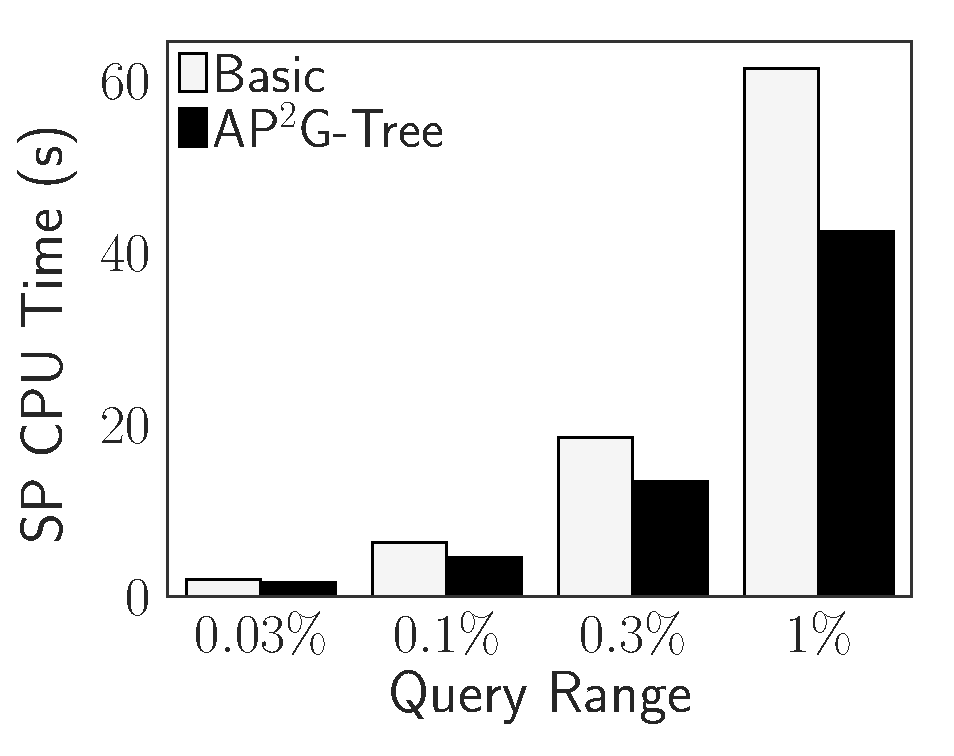
\includegraphics[width=.33\linewidth]{exp-figs/access-control/range_sp.eps}%
}

\begin{figure}[t]
    \centering
    \begin{subfigure}{.33\linewidth}
        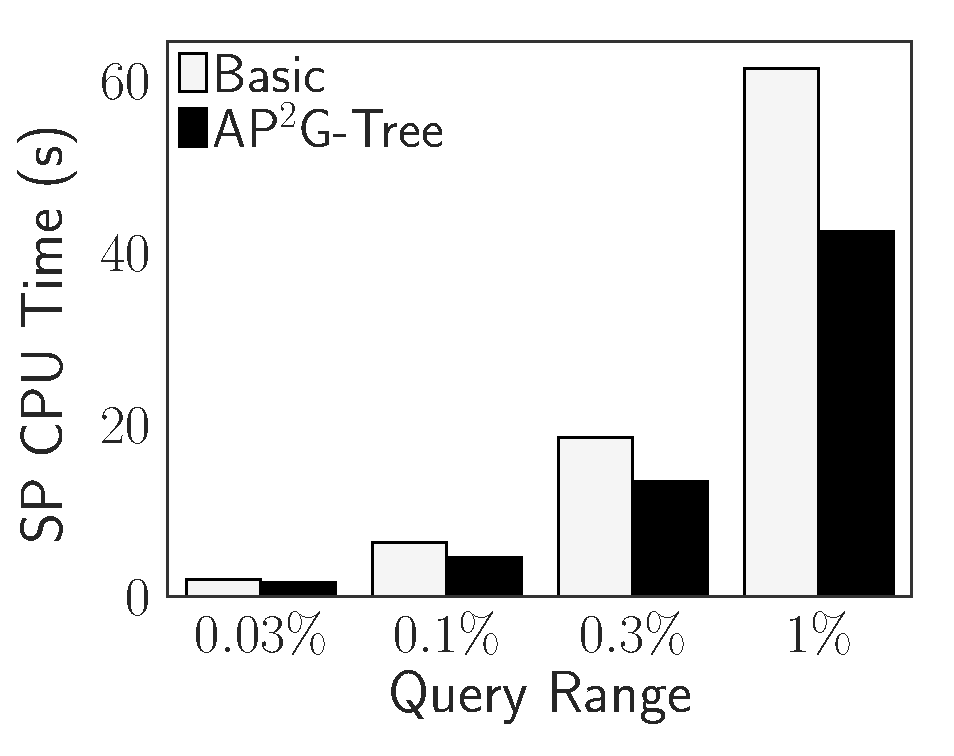
\includegraphics[height=\ht\figbox]{exp-figs/access-control/range_sp.eps}
        \caption{SP CPU Time}
    \end{subfigure}~%
    \begin{subfigure}{.33\linewidth}
        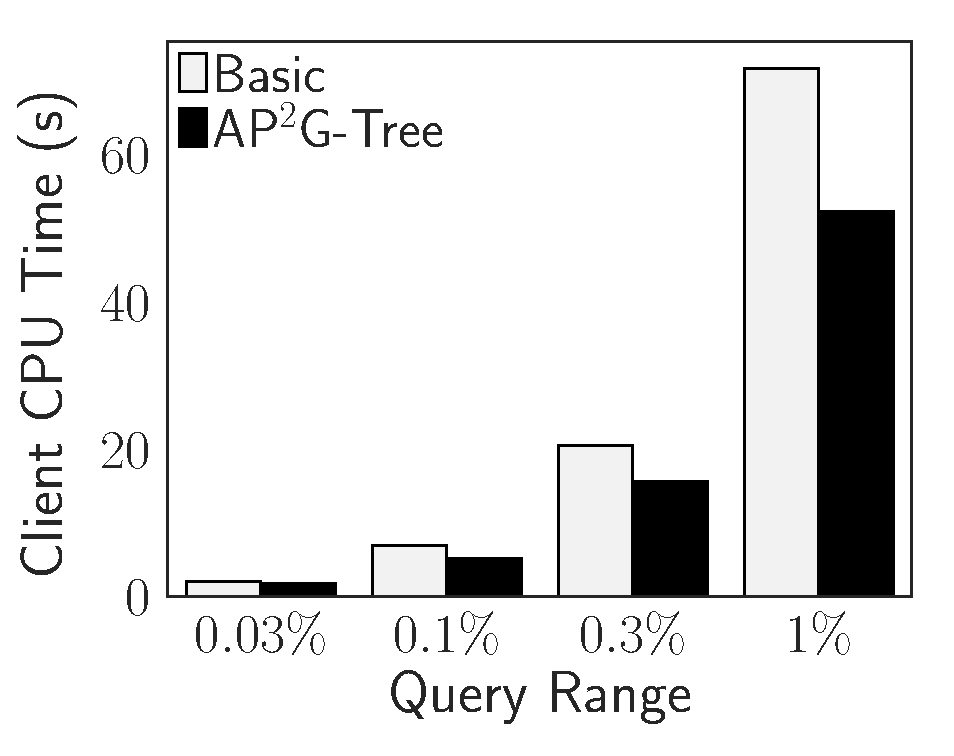
\includegraphics[height=\ht\figbox]{exp-figs/access-control/range_user.eps}
        \caption{Client CPU Time}
    \end{subfigure}~%
    \begin{subfigure}{.33\linewidth}
        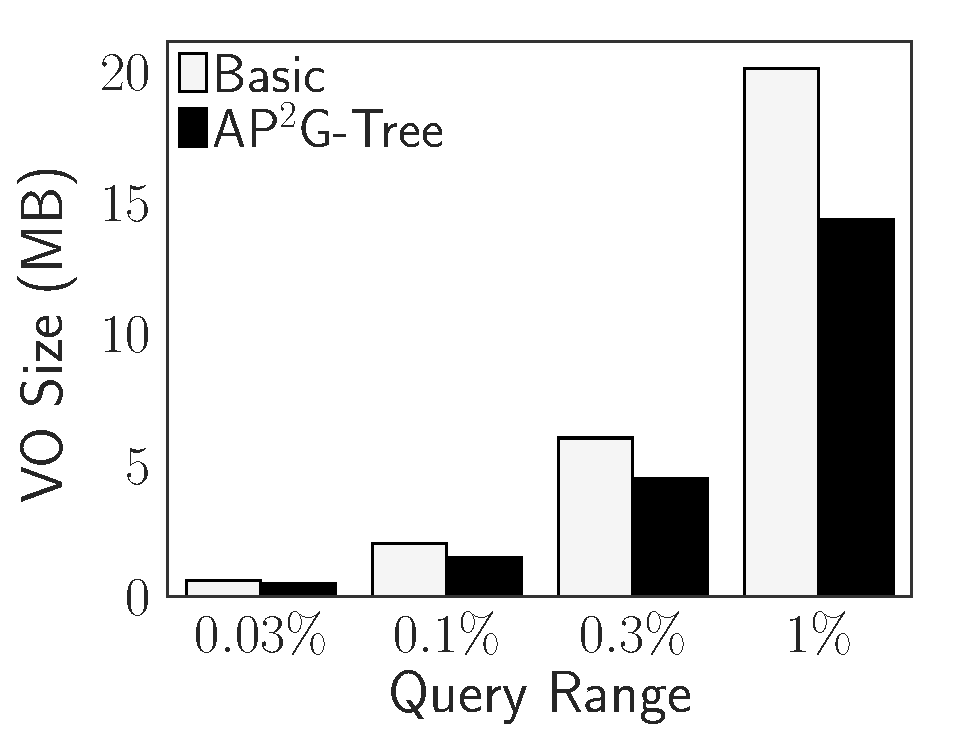
\includegraphics[height=\ht\figbox]{exp-figs/access-control/range_vo.eps}
        \caption{VO Size}
    \end{subfigure}
    \caption{Range Query Performance vs. Range}\label{exp-fig:access-control:range}
\end{figure}
\begin{figure}[t]
    \centering
    \begin{subfigure}{.33\linewidth}
        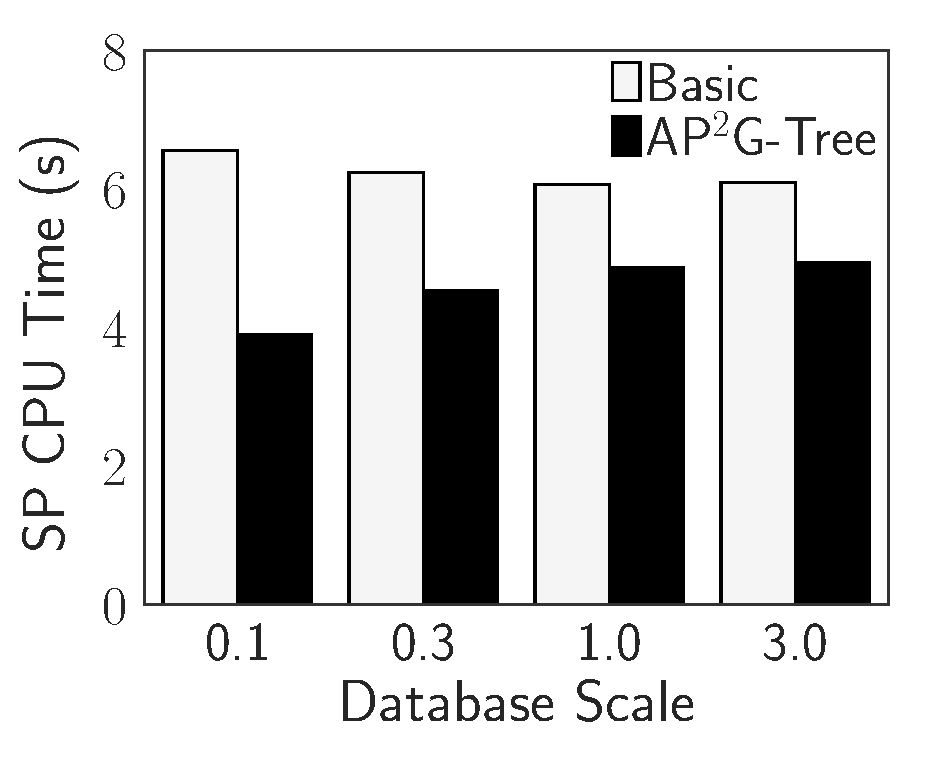
\includegraphics[height=\ht\figbox]{exp-figs/access-control/scale_sp.eps}
        \caption{SP CPU Time}
    \end{subfigure}~%
    \begin{subfigure}{.33\linewidth}
        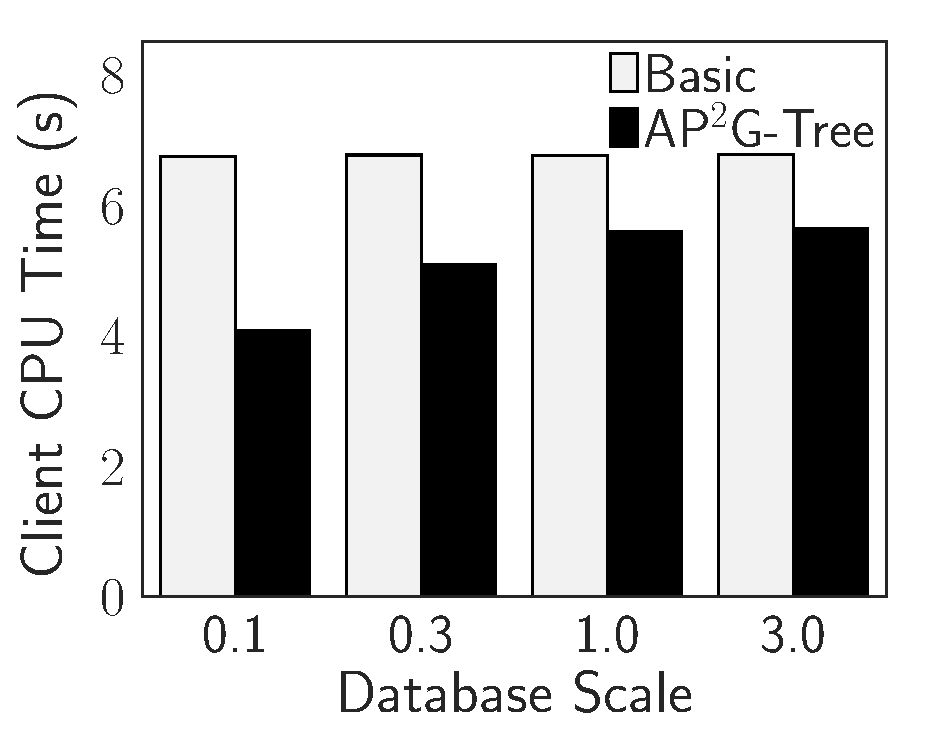
\includegraphics[height=\ht\figbox]{exp-figs/access-control/scale_user.eps}
        \caption{Client CPU Time}
    \end{subfigure}~%
    \begin{subfigure}{.33\linewidth}
        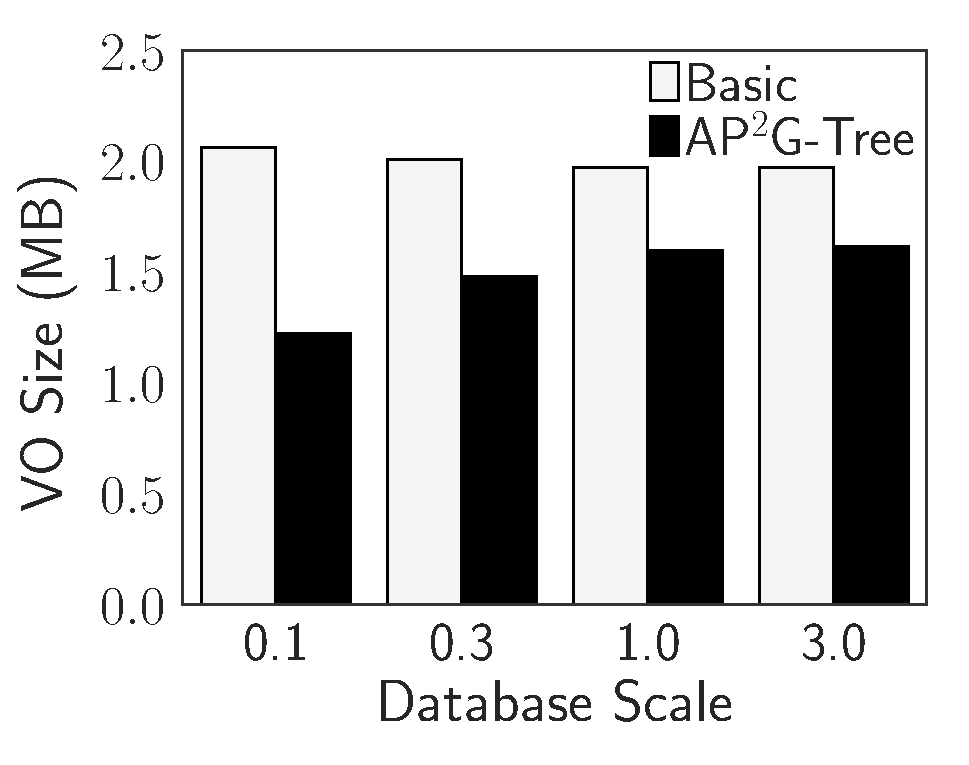
\includegraphics[height=\ht\figbox]{exp-figs/access-control/scale_vo.eps}
        \caption{VO Size}\label{exp-fig:scale_vo}
    \end{subfigure}
    \caption{Range Query Performance vs. Database Scale}\label{exp-fig:access-control:scale}
\end{figure}
\begin{figure}[t]
    \centering
    \begin{subfigure}{.33\linewidth}
        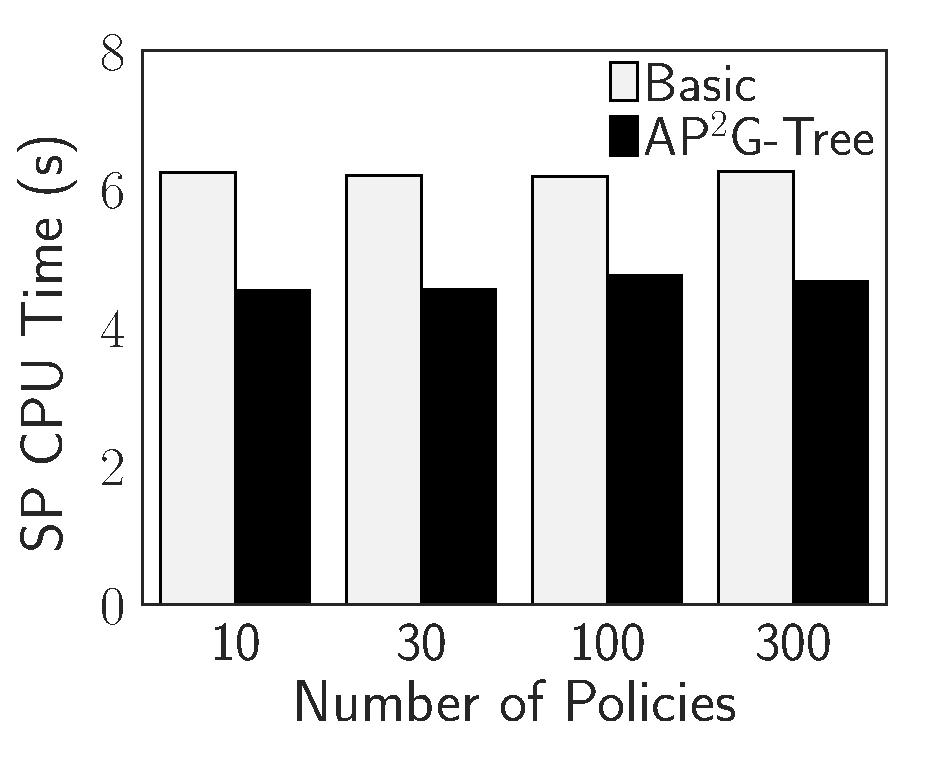
\includegraphics[height=\ht\figbox]{exp-figs/access-control/policy_1_sp.eps}
        \caption{SP CPU Time}
    \end{subfigure}~%
    \begin{subfigure}{.33\linewidth}
        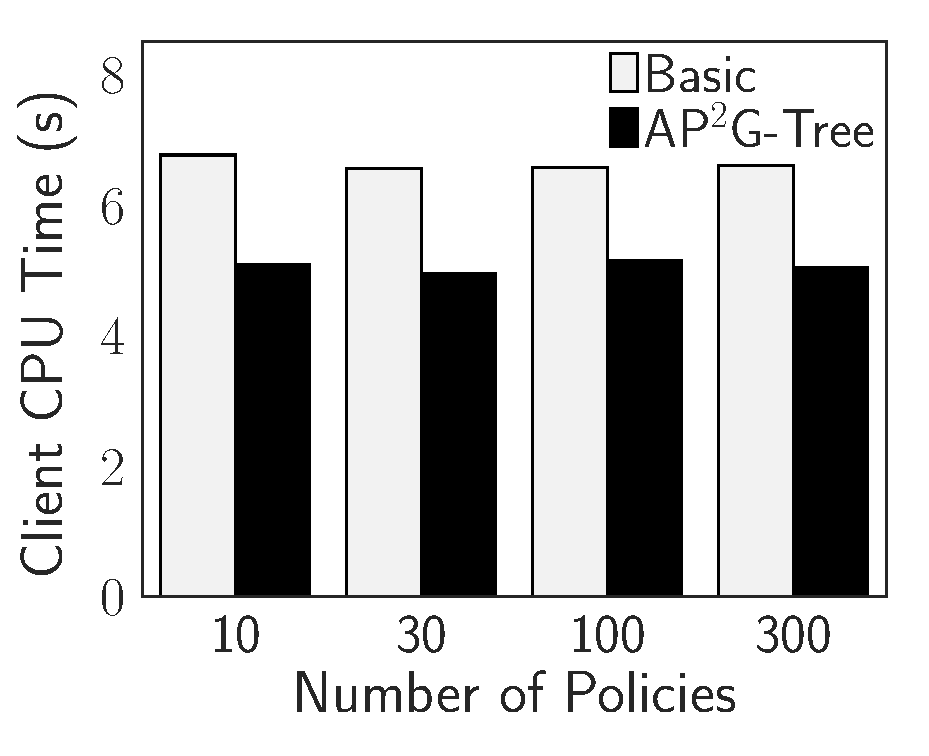
\includegraphics[height=\ht\figbox]{exp-figs/access-control/policy_1_user.eps}
        \caption{Client CPU Time}
    \end{subfigure}~%
    \begin{subfigure}{.33\linewidth}
        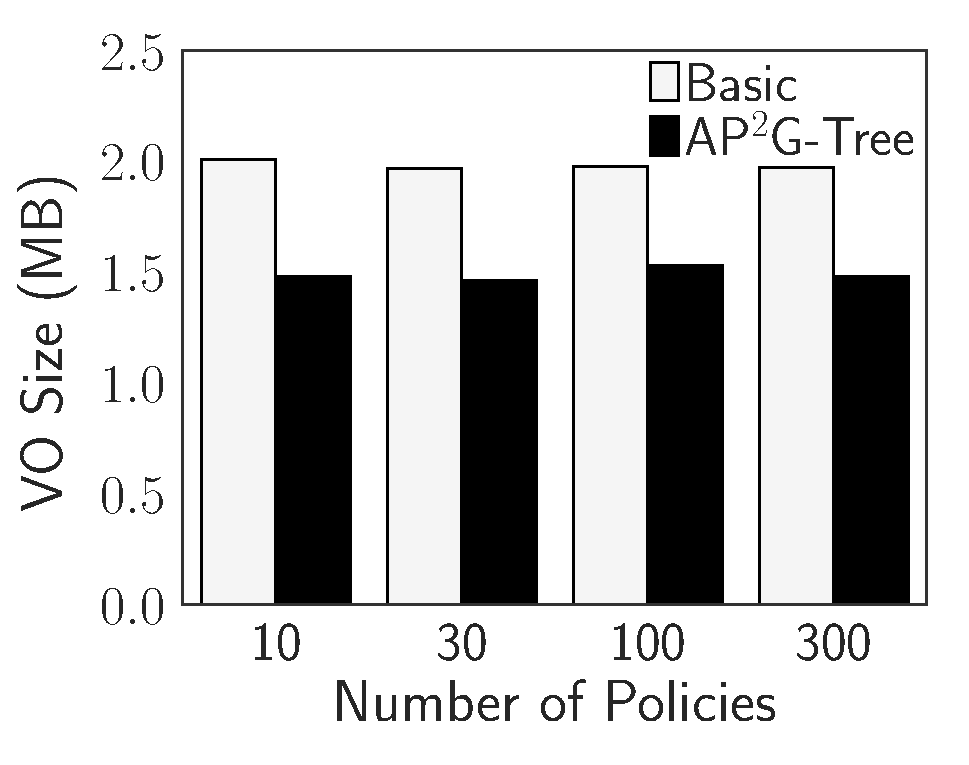
\includegraphics[height=\ht\figbox]{exp-figs/access-control/policy_1_vo.eps}
        \caption{VO Size}
    \end{subfigure}
    \caption{Range Query Performance vs. Policy Diversity}\label{exp-fig:access-control:policy_1}
\end{figure}
\begin{figure}[t]
    \centering
    \begin{subfigure}{.33\linewidth}
        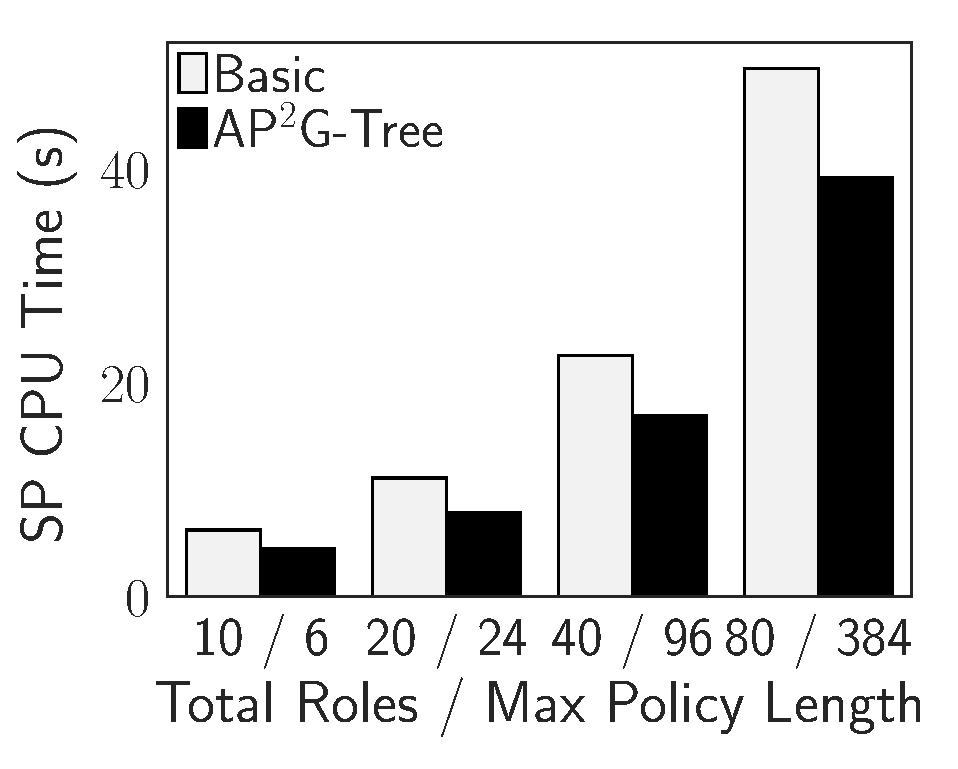
\includegraphics[height=\ht\figbox]{exp-figs/access-control/policy_2_sp.eps}
        \caption{SP CPU Time}
    \end{subfigure}~%
    \begin{subfigure}{.33\linewidth}
        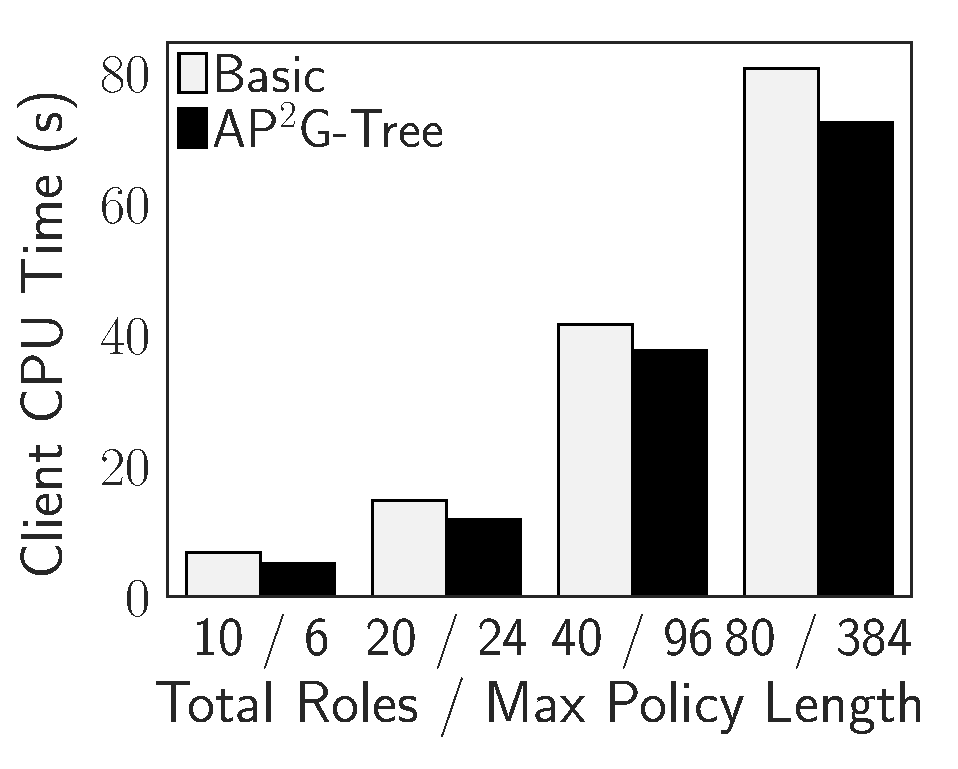
\includegraphics[height=\ht\figbox]{exp-figs/access-control/policy_2_user.eps}
        \caption{Client CPU Time}
    \end{subfigure}~%
    \begin{subfigure}{.33\linewidth}
        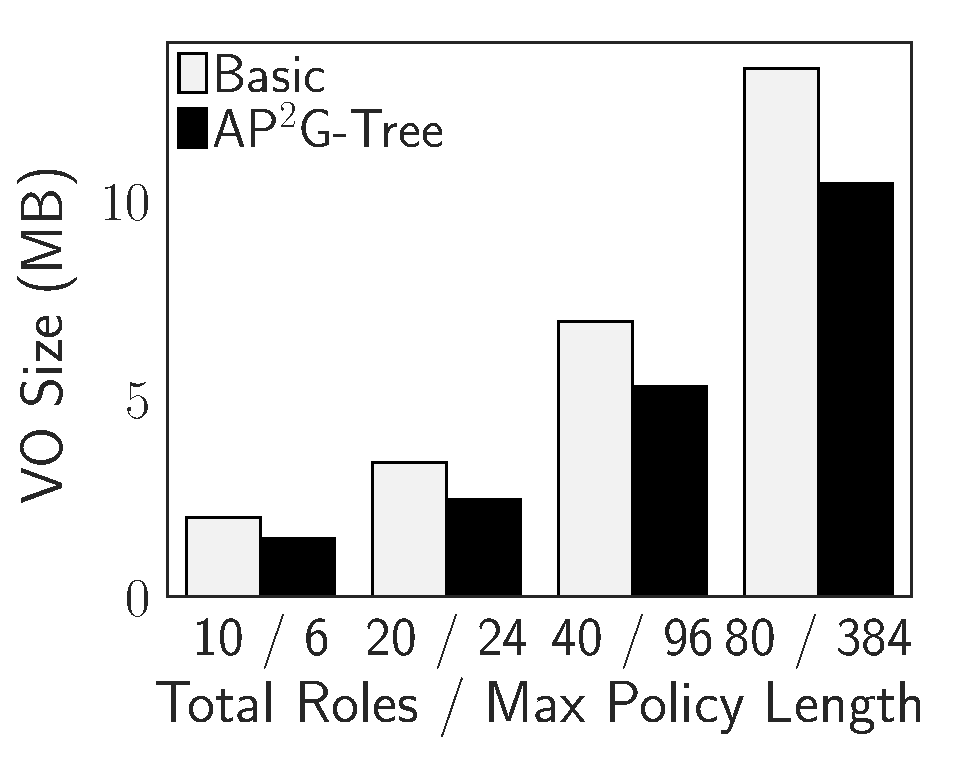
\includegraphics[height=\ht\figbox]{exp-figs/access-control/policy_2_vo.eps}
        \caption{VO Size}
    \end{subfigure}
    \caption{Range Query Performance vs. Total Roles}\label{exp-fig:access-control:policy_2}
\end{figure}
\begin{figure}[t]
    \centering
    \begin{subfigure}{.33\linewidth}
        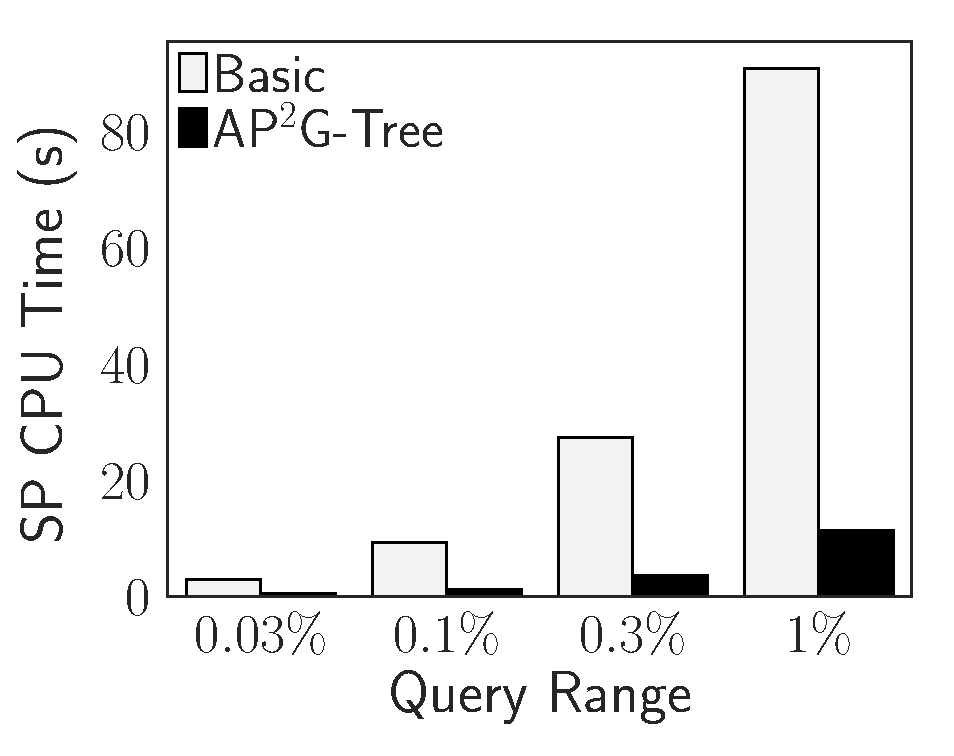
\includegraphics[height=\ht\figbox]{exp-figs/access-control/join_sp.eps}
        \caption{SP CPU Time}
    \end{subfigure}~%
    \begin{subfigure}{.33\linewidth}
        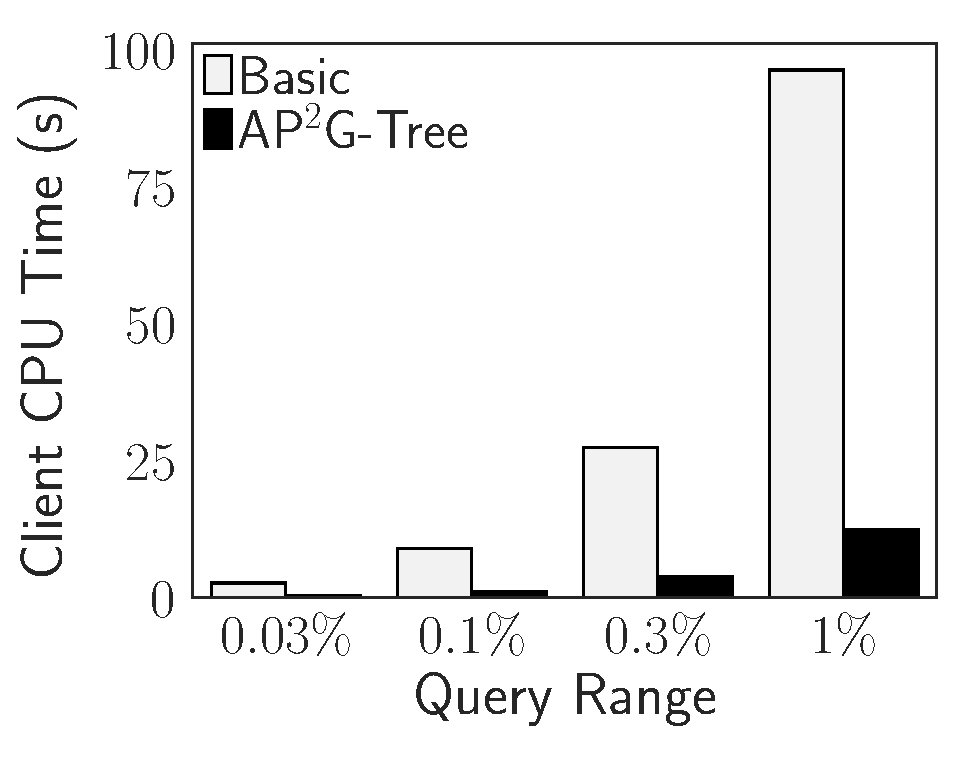
\includegraphics[height=\ht\figbox]{exp-figs/access-control/join_user.eps}
        \caption{Client CPU Time}
    \end{subfigure}~%
    \begin{subfigure}{.33\linewidth}
        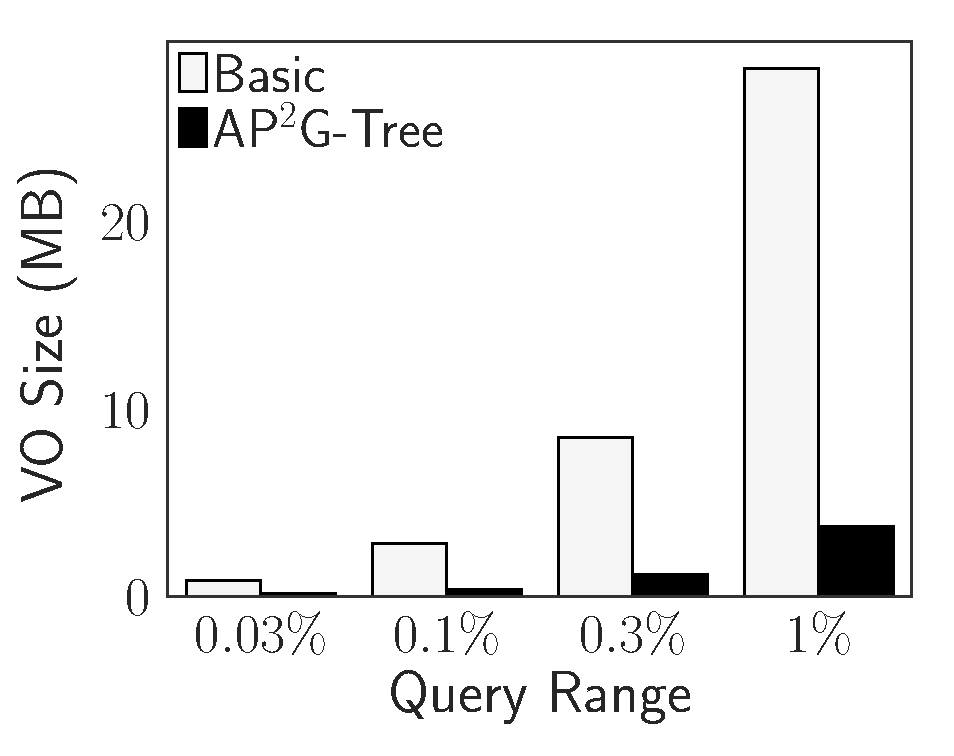
\includegraphics[height=\ht\figbox]{exp-figs/access-control/join_vo.eps}
        \caption{VO Size}
    \end{subfigure}
    \caption{Join Query Performance vs. Range}\label{exp-fig:access-control:join}
\end{figure}

To evaluate the range query authentication performance, we compare two methods:
\begin{inlineenum}
    \item the basic approach in which equality query authentication is executed repeatedly for every discrete value lying in the query range, and
    \item the AP$^2$G-tree approach developed in \cref{sec:access-control:range-query}.
\end{inlineenum}
In each query, the client is assigned with the roles that can access 20\% of the data records.

We first vary the query range from 0.03\% to 1\% of the data space under the default settings. As shown in \cref{exp-fig:access-control:range}, the AP$^2$G-tree outperforms the basic approach in all metrics. This indicates that the APS signatures generated for AP$^2$G-tree nodes can effectively summarize the inaccessible records in their subtrees. This leads to the reduction in both computation and communication overheads.

To investigate the impact of the database scale and access policies, we fix the query range at 0.1\%. \Cref{exp-fig:access-control:scale} shows the results when the database scale is varied from 0.1 to 3. All metrics increase monotonically under AP$^2$G-tree, but those of the basic approach fluctuate a bit. This can be explained as follows. With more records, the access policies become more complex. This affects the costs in two ways:
\begin{inlineenum}
    \item it takes the SP more time to process the \textsf{ABS.Relax} operations, and
    \item it takes the client more time to verify the APP signatures.
\end{inlineenum}
On the other hand, with the increase of database scale, more records can be accessed by the client and, hence, the inaccessible records become fewer. This decreases the costs on both the SP and the client.
For AP$^2$G-tree, owing to its high pruning power, the decreased number of inaccessible records has less impact on the costs. Therefore, its costs increase steadily.

\Cref{exp-fig:access-control:policy_1} and~\cref{exp-fig:access-control:policy_2} show the performance trends with the respect to the number of distinct policies and the total number of roles/max policy length, respectively. It can be seen that the performance remains almost the same under different policy diversities. However, the larger the role space and the longer access policy length, the higher the overhead incurred for both the computation and communication costs.

Finally, to study the join query performance, we evaluate the join operator of $Q$12 in TPC-H,\footnote{\texttt{SELECT * FROM orders, lineitem WHERE o.orderkey = l.orderkey AND l.orderkey between `?' AND `?'.}} which joins the tables \texttt{Lineitem} and \texttt{Orders} on the attribute $orderkey$. \Cref{exp-fig:access-control:join} reports the results while varying the query range. It is shown that the costs in all metrics under AP$^2$G-tree are substantially lower than those in the basic approach.

\subsection{Impact of the Optimizations}

\begin{figure}[t]
    \centering
    \begin{subfigure}{.33\linewidth}
        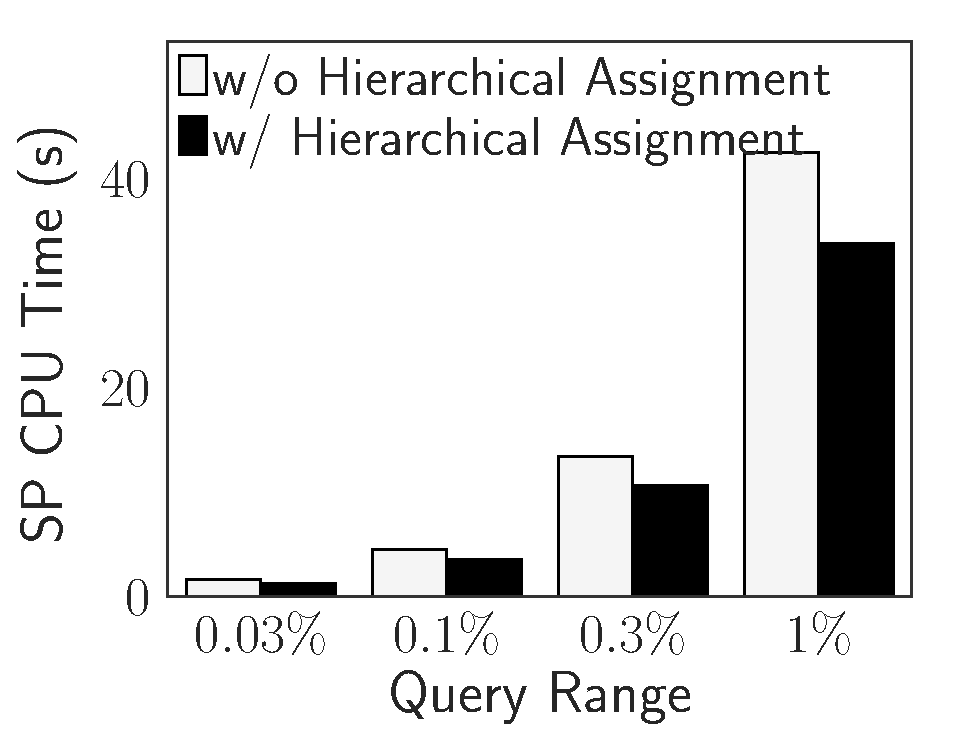
\includegraphics[height=\ht\figbox]{exp-figs/access-control/hierarchical_sp.eps}
        \caption{SP CPU Time}
    \end{subfigure}~%
    \begin{subfigure}{.33\linewidth}
        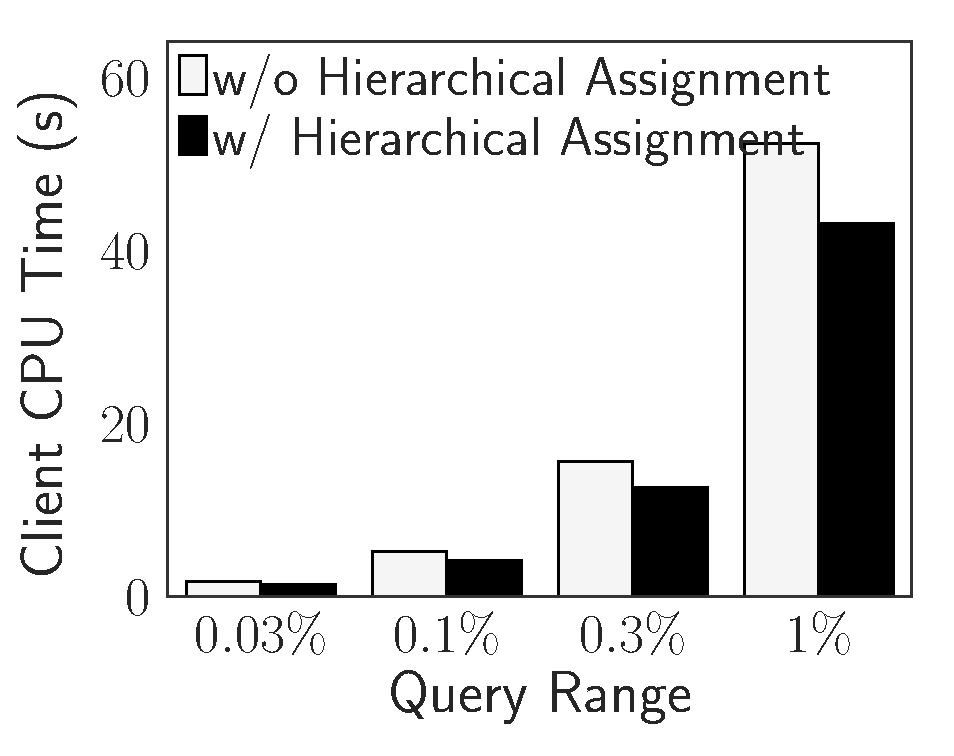
\includegraphics[height=\ht\figbox]{exp-figs/access-control/hierarchical_user.eps}
        \caption{Client CPU Time}
    \end{subfigure}~%
    \begin{subfigure}{.33\linewidth}
        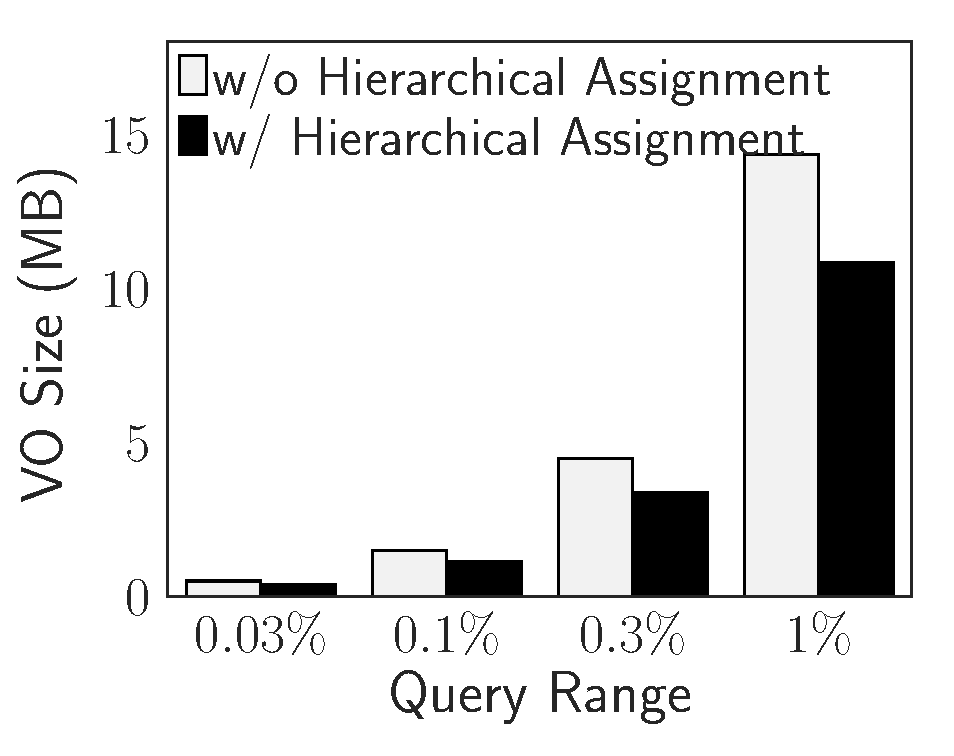
\includegraphics[height=\ht\figbox]{exp-figs/access-control/hierarchical_vo.eps}
        \caption{VO Size}
    \end{subfigure}
    \caption{Hierarchical Role Assignment Acceleration}\label{exp-fig:access-control:hierarchical}
\end{figure}
\begin{figure}[t]
    \centering
    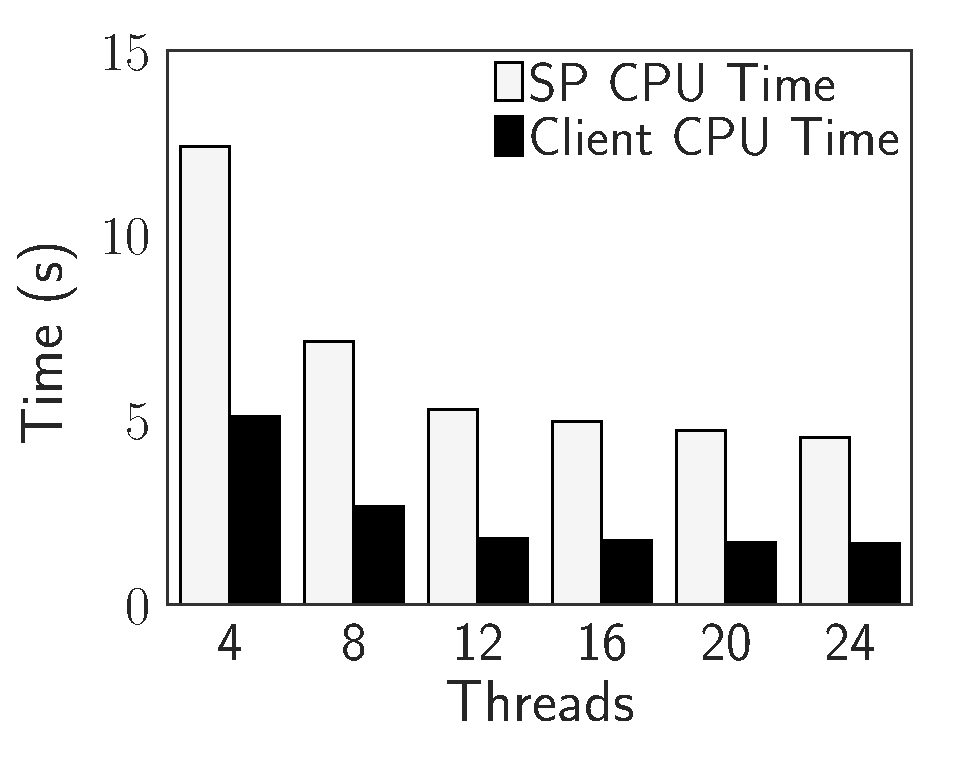
\includegraphics[height=\ht\figbox]{exp-figs/access-control/thread.eps}
    \caption{Multi-Threaded Acceleration}\label{exp-fig:access-control:thread}
\end{figure}
\begin{figure}[t]
    \centering
    \begin{subfigure}{.33\linewidth}
        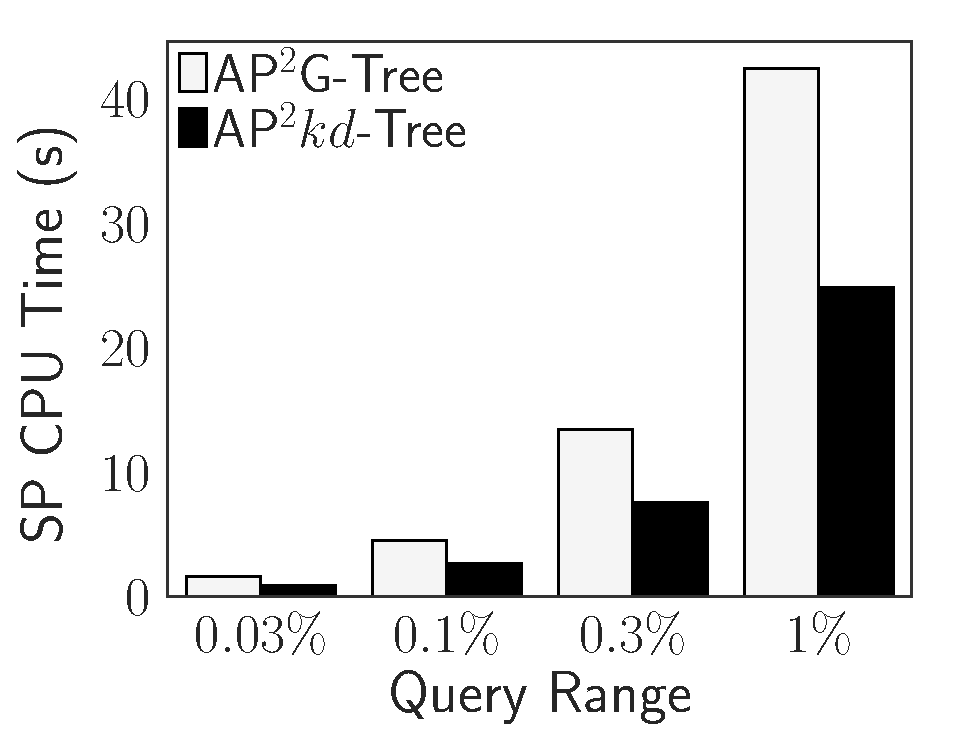
\includegraphics[height=\ht\figbox]{exp-figs/access-control/index_1_sp.eps}
        \caption{SP CPU Time}
    \end{subfigure}~%
    \begin{subfigure}{.33\linewidth}
        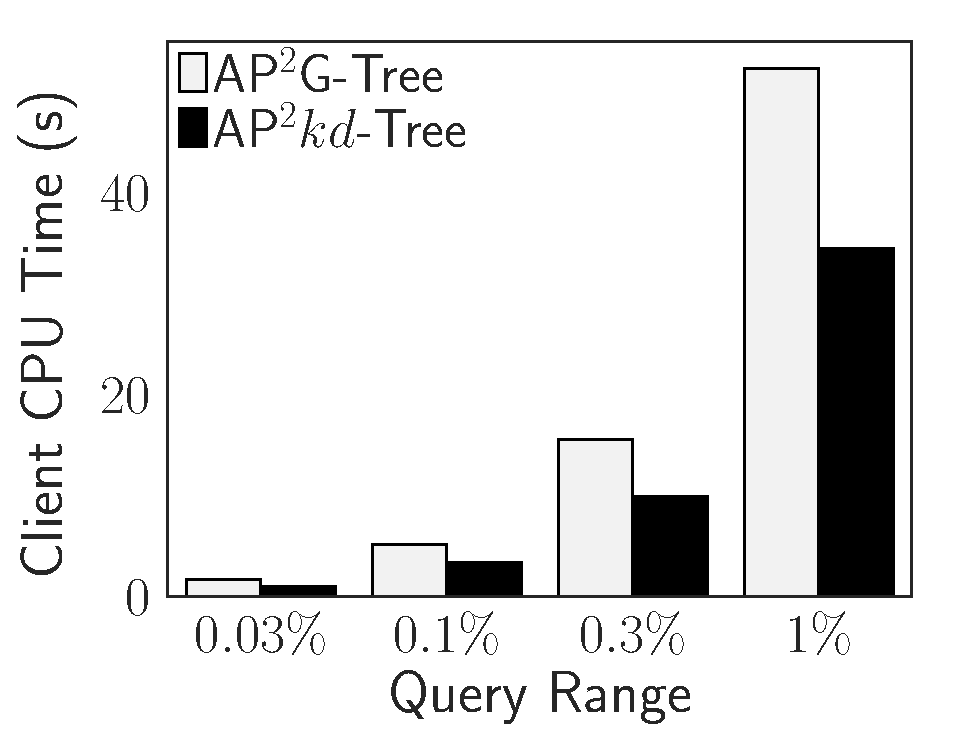
\includegraphics[height=\ht\figbox]{exp-figs/access-control/index_1_user.eps}
        \caption{Client CPU Time}
    \end{subfigure}~%
    \begin{subfigure}{.33\linewidth}
        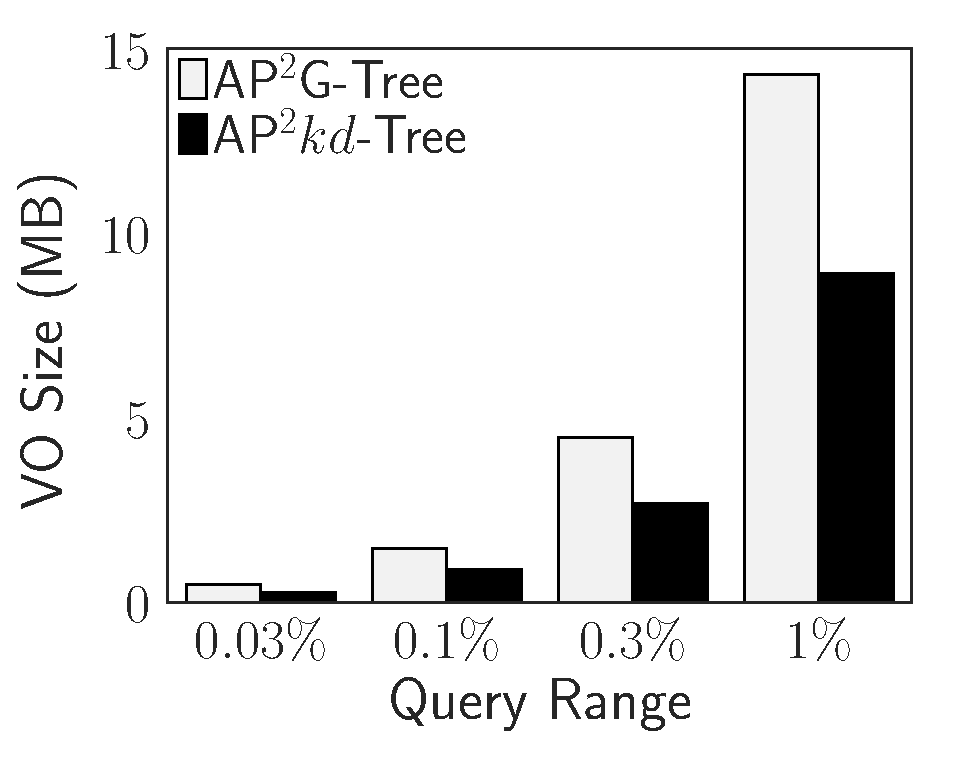
\includegraphics[height=\ht\figbox]{exp-figs/access-control/index_1_vo.eps}
        \caption{VO Size}
    \end{subfigure}
    \caption{Range Query Performance vs. Index}\label{exp-fig:access-control:index}
\end{figure}

We now investigate the impact of different optimization techniques proposed in \cref{sec:access-control:opt}. The results of using hierarchical role assignment are shown in \cref{exp-fig:access-control:hierarchical}. In our experiment, we simulate a two-level role hierarchy. Two global hierarchical roles are created and attached randomly to each AND gate in all the access policies. As a result, the average size of a client's inaccessible predicate is decreased from 9 to 6. It can be observed that the hierarchical role assignment reduces the cost in all metrics, due to much less overhead in processing inaccessible records.

To study the acceleration acquired by parallelism, we vary the number of threads for both the SP processing and client verification running on the blade server. As shown in \cref{exp-fig:access-control:thread}, more acceleration can be observed with the first 16 threads, but it becomes less effective with more threads. The reason is that the non-parallel part of the algorithm and I/O operations becomes more pronounced after sufficient multi-thread acceleration.

Finally, we study the performance gain if we relax the zero-knowledge confidentiality requirement. As shown in \cref{exp-fig:access-control:index}, owing to a careful splitting strategy introduced in \cref{sec:access-control:kd-tree}, AP$^2kd$-tree substantially outperforms AP$^2$G-tree in all evaluation metrics.

\subsection{Performance with Duplicate Records and Updates}

\begin{figure}[t]
    \centering
    \begin{subfigure}{.33\linewidth}
        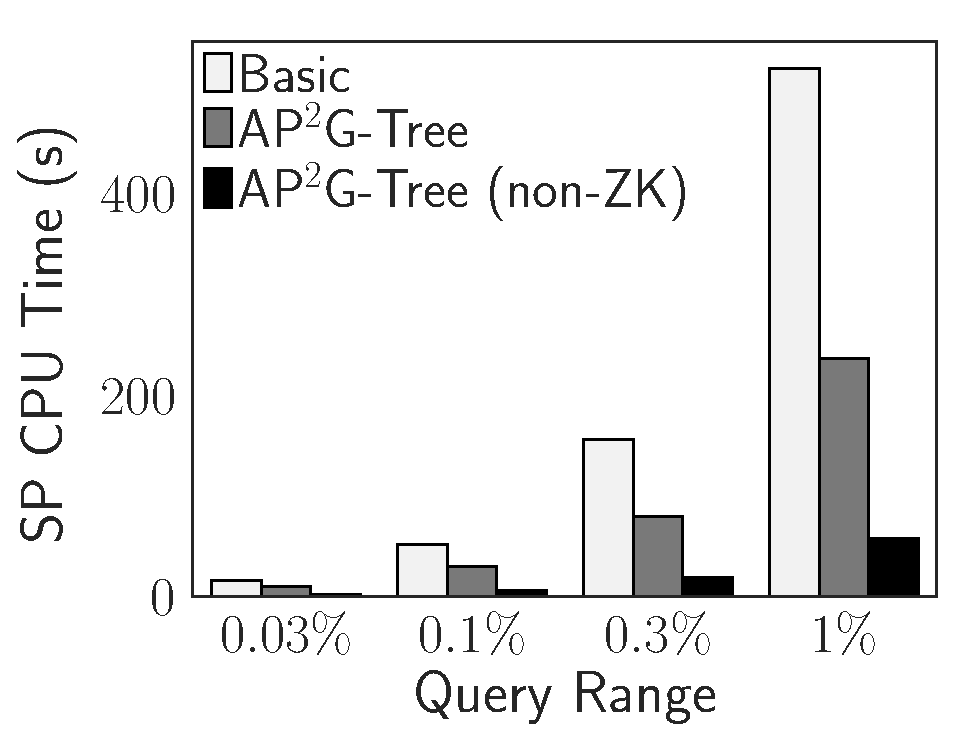
\includegraphics[height=\ht\figbox]{exp-figs/access-control/dup_sp.eps}
        \caption{SP CPU Time}
    \end{subfigure}~%
    \begin{subfigure}{.33\linewidth}
        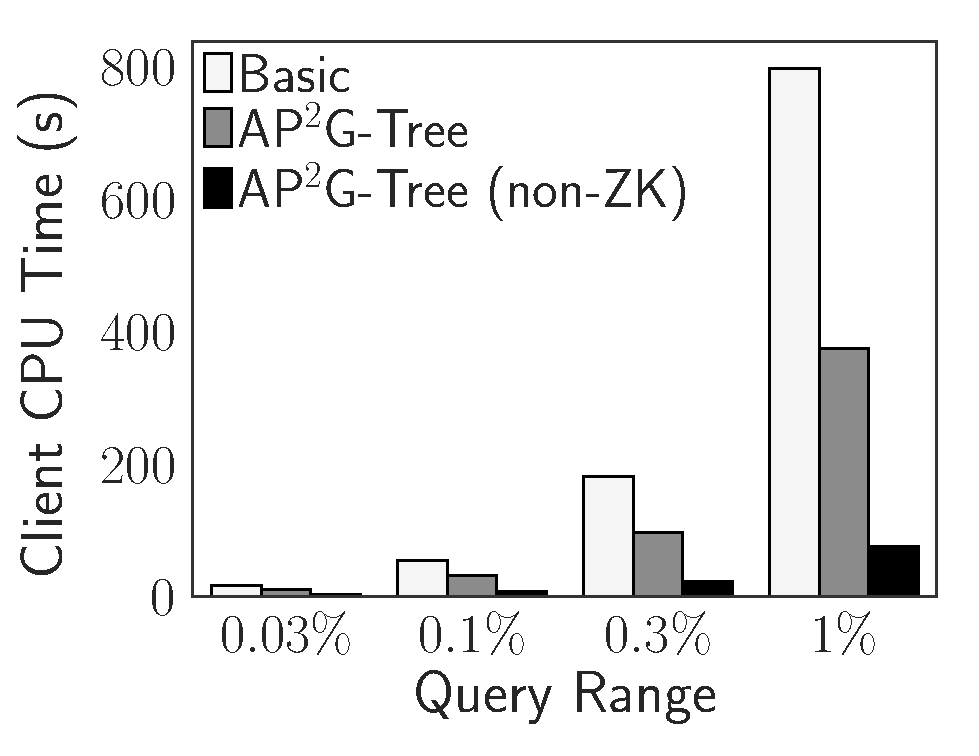
\includegraphics[height=\ht\figbox]{exp-figs/access-control/dup_user.eps}
        \caption{Client CPU Time}
    \end{subfigure}~%
    \begin{subfigure}{.33\linewidth}
        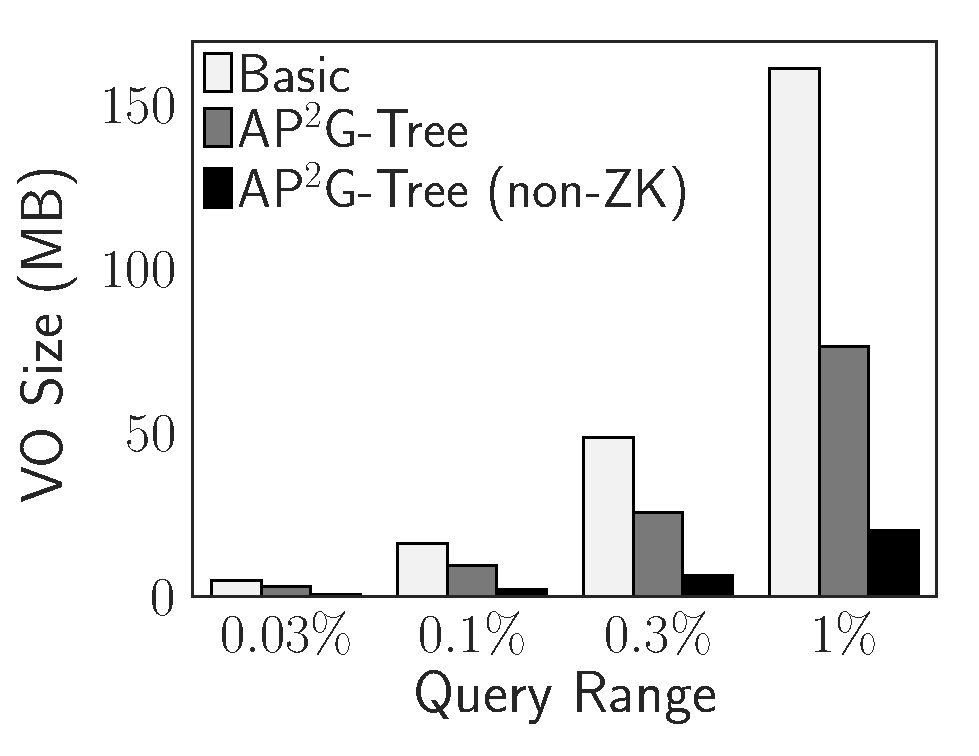
\includegraphics[height=\ht\figbox]{exp-figs/access-control/dup_vo.eps}
        \caption{VO Size}
    \end{subfigure}
    \caption{Range Query Performance with Duplicate Records}\label{exp-fig:access-control:dup}
\end{figure}

To investigate the performance with duplicate records using methods proposed in \cref{sec:access-control:dup}, we conduct performance evaluation over the default TPC-H database, where the access policies are randomly assigned to all data records.
We compare two solutions of handling duplicate records:
\begin{inlineenum}
    \item the zero-knowledge approach by adding the virtual dimension (denoted as AP$^2$G-Tree);
    \item the non-zero-knowledge approach by embedding the duplicate information in the APP signatures (denoted as AP$^2$G-Tree (non-ZK)).
\end{inlineenum}
The index size for the zero-knowledge approach is 12.17 GB (2.91 GB tree structure + 9.26 GB signatures), whereas in the non-zero-knowledge setting the index is 4.35 GB (1.02 GB tree structure + 3.33 GB signatures). The additional index overhead incurred for the zero-knowledge approach, as the cost of achieving the zero-knowledge requirement, is believed to be reasonable. Regarding the query performance, AP$^2$G-Tree (non-ZK) is approximate to the case without duplicate records since the duplicate information is seamlessly embedded in the APP signatures. As shown in \cref{exp-fig:access-control:dup}, the query cost in the zero-knowledge AP$^2$G-tree approach is only no more than 3 times worse than that in AP$^2$G-Tree (non-ZK). Moreover, the performance of AP$^2$G-tree is only about half that of the basic approach, which again demonstrates its pruning effectiveness for inaccessible records.

\begin{figure}[t]
    \centering
    \begin{subfigure}[b]{.5\linewidth}
        \centering
        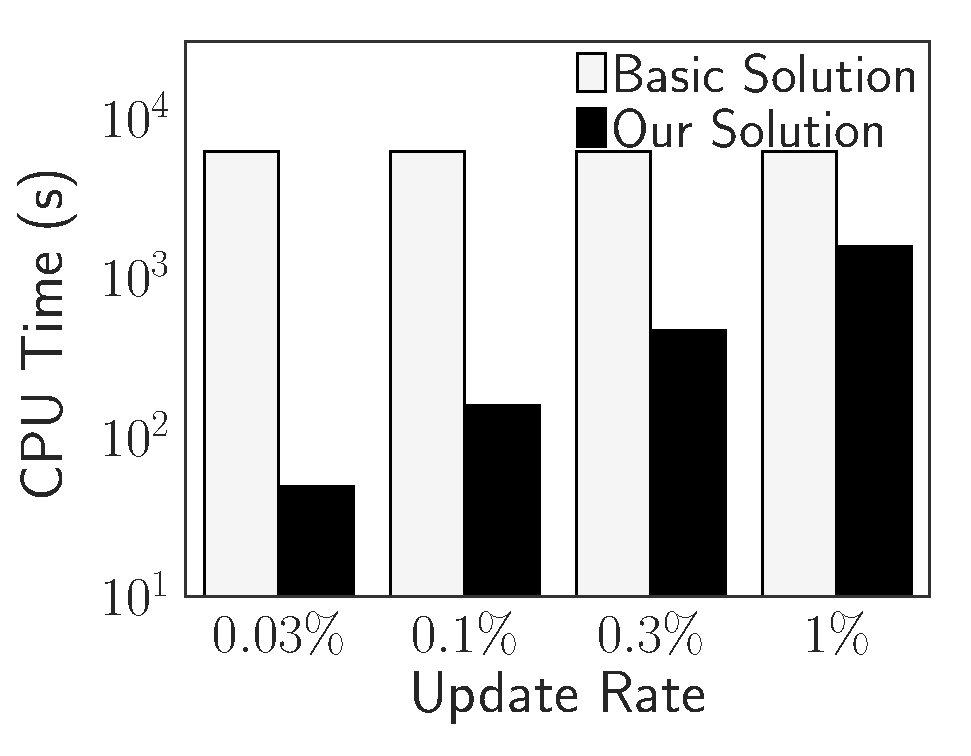
\includegraphics[height=\ht\figbox]{exp-figs/access-control/update_do_time.eps}
        \caption{DO CPU Time}\label{exp-fig:access-control:update_do_time}
    \end{subfigure}~%
    \begin{subfigure}[b]{.5\linewidth}
        \centering
        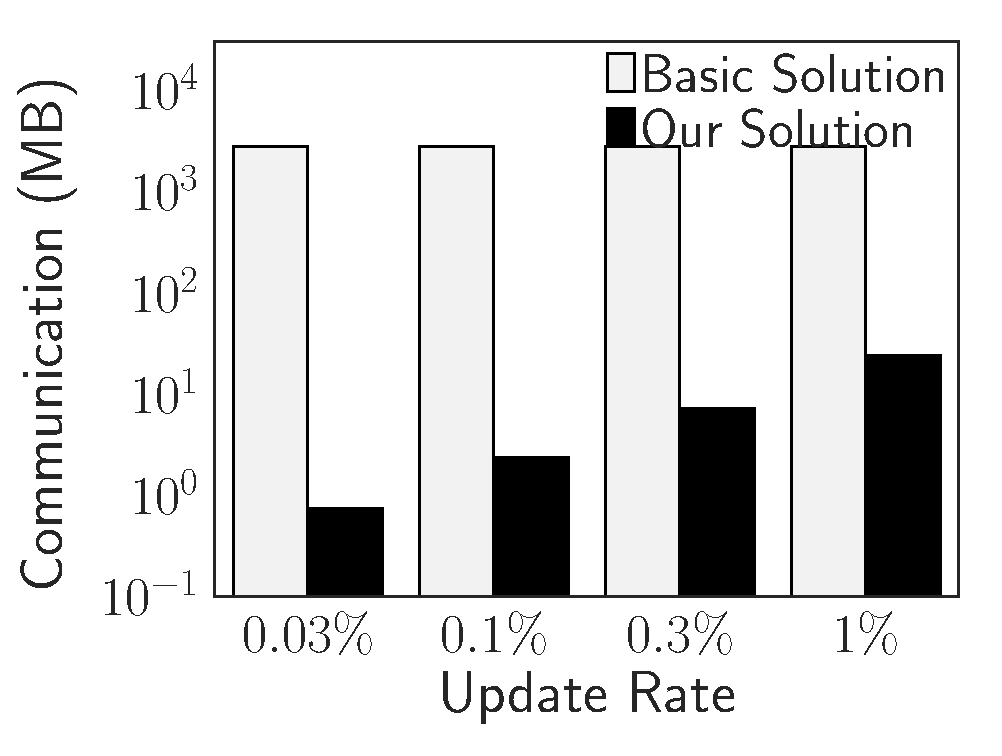
\includegraphics[height=\ht\figbox]{exp-figs/access-control/update_do_size.eps}
        \caption{Communication Cost}\label{exp-fig:access-control:update_do_size}
    \end{subfigure}
    \caption{Update Performance vs. Update Rate}\label{exp-fig:access-control:update_do}
\end{figure}
\begin{figure}[t]
    \centering
    \begin{subfigure}{.33\linewidth}
        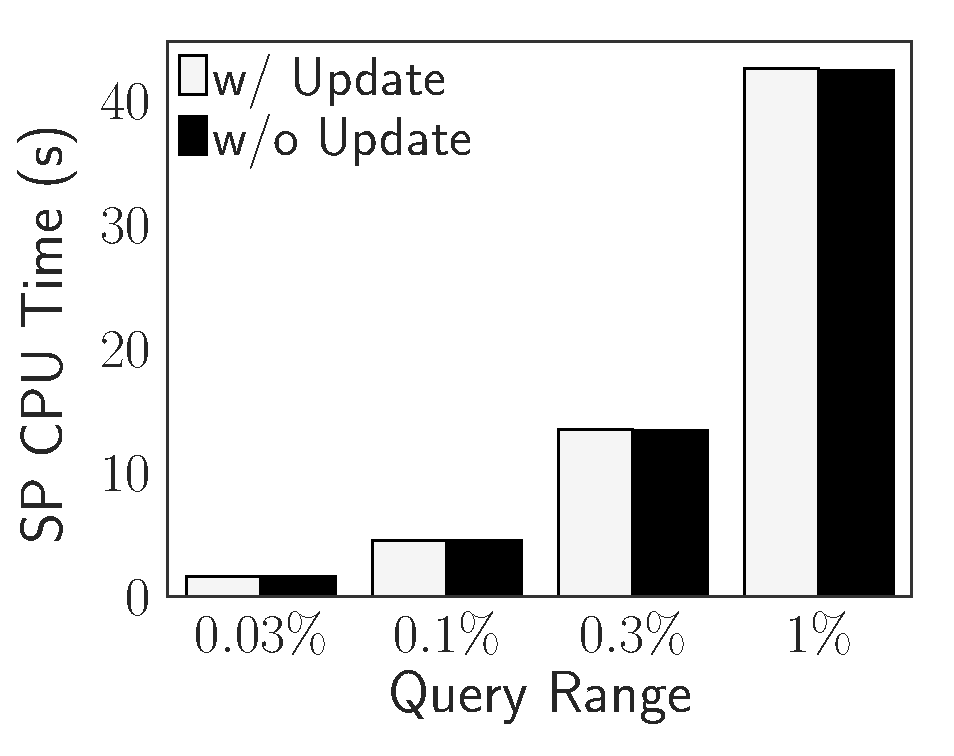
\includegraphics[height=\ht\figbox]{exp-figs/access-control/update_sp.eps}
        \caption{SP CPU Time}
    \end{subfigure}~%
    \begin{subfigure}{.33\linewidth}
        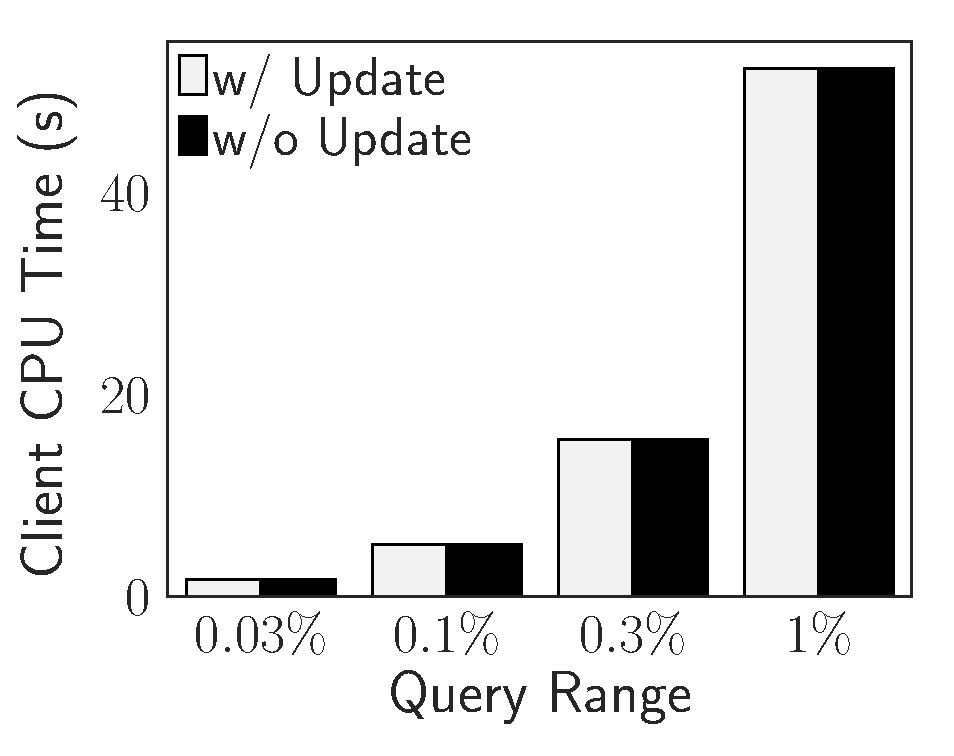
\includegraphics[height=\ht\figbox]{exp-figs/access-control/update_user.eps}
        \caption{Client CPU Time}
    \end{subfigure}~%
    \begin{subfigure}{.33\linewidth}
        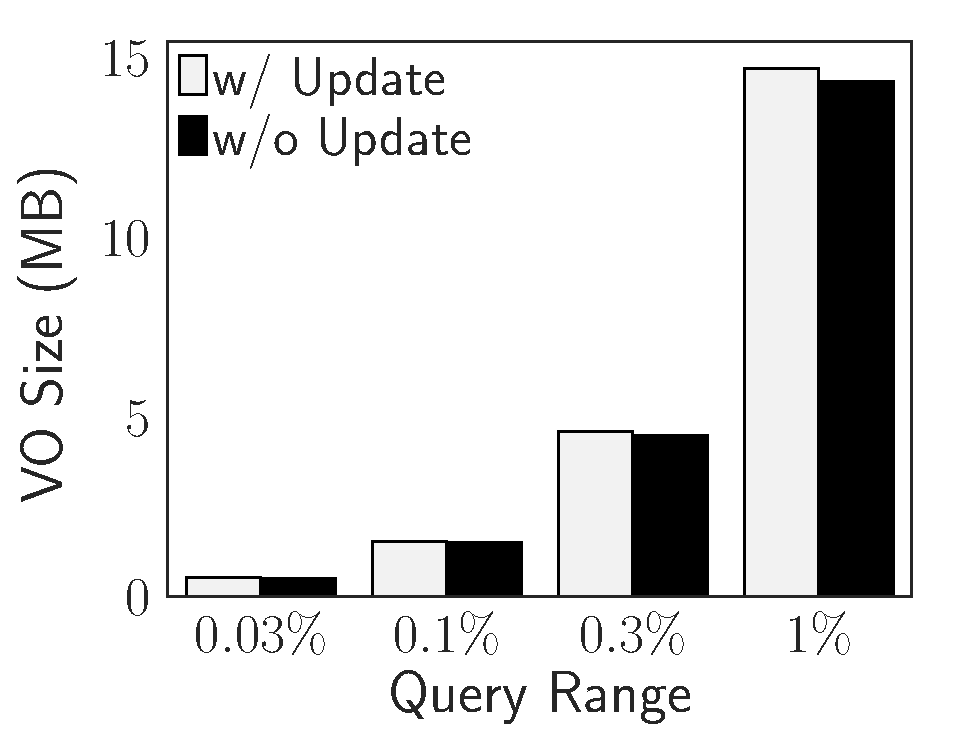
\includegraphics[height=\ht\figbox]{exp-figs/access-control/update_vo.eps}
        \caption{VO Size}
    \end{subfigure}
    \caption{Range Query Performance vs. Update}\label{exp-fig:access-control:update}
\end{figure}

Finally, we conduct an empirical study over the default TPC-H database to evaluate the performance of our update strategy proposed in \cref{sec:access-control:update}. We compare two update methods:
\begin{inlineenum}
    \item the basic approach in which the DO resigns all of the APP signatures; and
    \item our proposed solution described above.
\end{inlineenum}
\Cref{exp-fig:access-control:update_do} reports the DO CPU time and the communication cost while varying the update rate from $0.03\%$ to $1\%$ of all the records. It can be observed that our solution is significantly better than the basic approach. Further, we study the performance differences of authenticating range queries with and without data record updates. As shown in \cref{exp-fig:access-control:update}, the differences in all metrics are insignificant.

\section{Chapter Summary}\label{sec:access-control:summary}
In this chpater, we have studied the problem of authenticating relational queries with fine-grained access control. We developed a new variant of the attribute-based signature scheme, which supports predicate relaxation on super access policies. Based on that, we proposed a novel access-policy-preserving (APP) signature as the primitive ADS to authenticate various types of queries under fine-grained access control. Our approach is zero-knowledge and reveals nothing beyond the accessible records. We also designed a grid-index-based AP$^2$G-tree to improve the performance of processing range queries and join queries. Optimization techniques for both the zero-knowledge model and the access policy confidentiality model were developed. Analytical models and empirical results substantiated the robustness and efficiency of our proposed solutions.
